\chapter{动力系统}
\label{cha:Motor}

注:微型反折步进电机和38mm全向轮之间联轴器上的螺丝配的是M3*4的圆头螺钉,在电机旋转时会碰到电机机身卡住,故换成M3*3的PM圆头螺丝。

\section{步进电机概述和控制理论}

\footnote{参考\url{https://www.moons.com.cn/support-training/technology-college/cn-stepper-motor}}

步进电机是将电脉冲信号转变为角位移或线位移的开环控制元步进电机件,通过控制施加在电机线圈上的电脉冲顺序、频率和数量,可以实现对步进电机的转向、速度和旋转角度的控制。配合以直线运动执行机构或齿轮箱装置,更可以实现更加复杂、精密的线性运动控制要求。步进电机一般由前后端盖、轴承、中心轴、转子铁芯、定子铁芯、定子组件、波纹垫圈、螺钉等部分构成,步进电机也叫步进器,它利用电磁学原理,将电能转换为机械能,是由缠绕在电机定子齿槽上的线圈驱动的。通常情况下,一根绕成圈状的金属丝叫做螺线管,而在电机中,绕在定子齿槽上的金属丝则叫做绕组、线圈、或相。如图~\ref{fig:Stepper-Motor-Open}。

\begin{figure}[htbp]
    \centering
    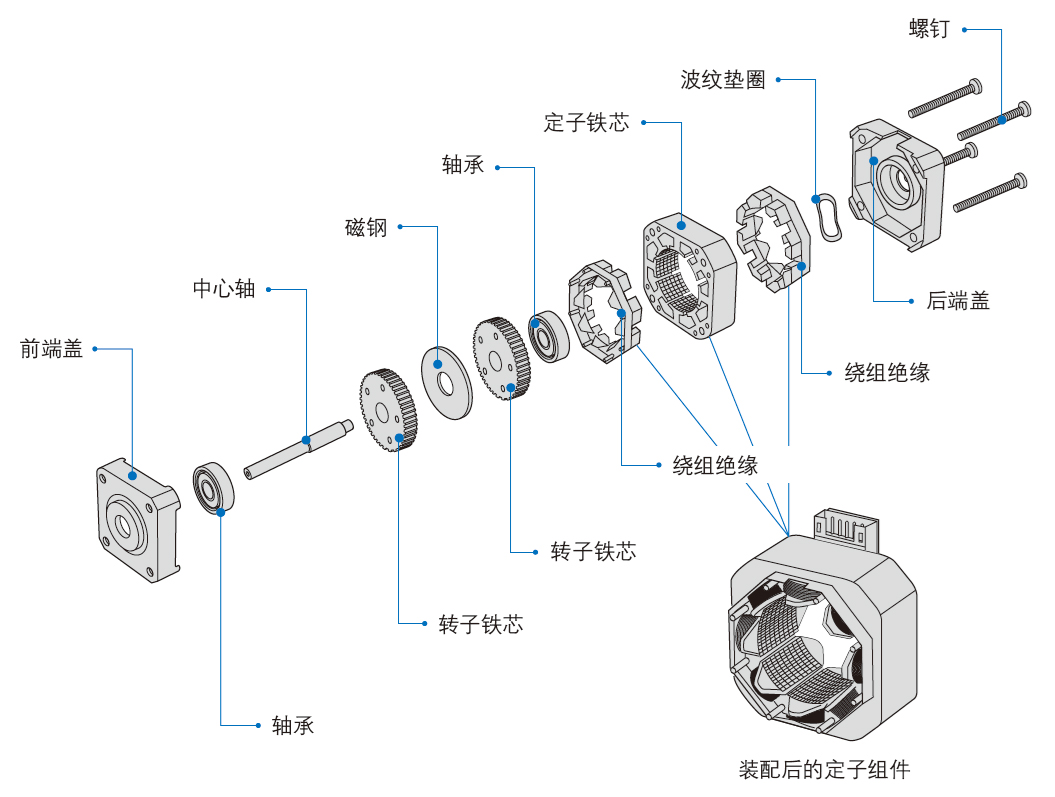
\includegraphics[width=\columnwidth]{step-servo-motord01.jpg}
    \caption{步进电机基本结构}
    \label{fig:Stepper-Motor-Open}
\end{figure}

步进电机驱动器根据外来的控制脉冲和方向信号,通过其内部的逻辑电路,控制步进电机的绕组以一定的时序正向或反向通电, 使得电机正向/反向旋转,或者锁定。

以1.8度两相步进电机为例:当两相绕组都通电励磁时,电机输出轴将静止并锁定位置。在额定电流下使电机保持锁定的最大力矩为保持力矩。如果其中一相绕组的电流发生了变向,则电机将顺着一个既定方向旋转一步(1.8度)。同理,如果是另外一项绕 组的电流发生了变向,则电机将顺着与前者相反的方向旋转一步(1.8度)。当通过线圈绕组的电流按顺序依次变向励磁时,则电 机会顺着既定的方向实现连续旋转步进,运行精度非常高。对于 1.8度两相步进电机旋转一周需200步。

两相步进电机有两种绕组形式:双极性和单极性。双极性电机每相上只有一个绕组线圈,电机连续旋转时电流要在 同一线圈内依次变向励磁,驱动电路设计上需要八个电子开关进 行顺序切换。

单极性电机每相上有两个极性相反的绕组线圈,如图~\ref{fig:bipolar},电机连续旋转时只要交替对同一相上的两个绕组线圈进行通电励磁。驱动电路设 计上只需要四个电子开关。在双极性驱动模式下,如图~\ref{fig:unipolar},因为每相的绕组线圈为100\%励磁,所以双极性驱动模式下电机的输出力矩比单极性驱动模式下提高了约 40\%。

\begin{figure}[htbp]
    \begin{minipage}{0.48\textwidth}
      \centering
      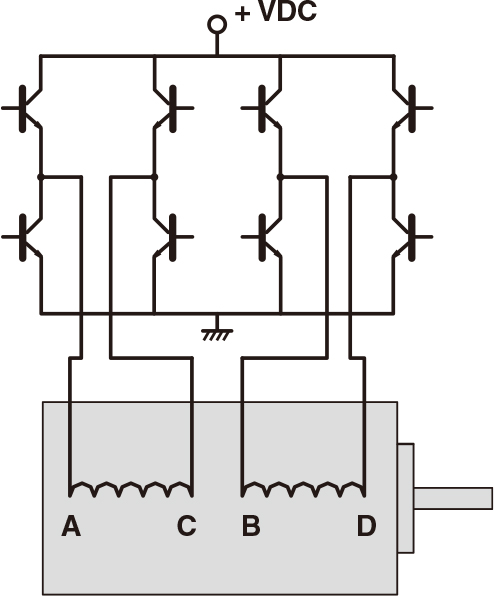
\includegraphics[height=5cm]{step-motor-2-phase-with-bipolar-driver.jpg}
      \caption{2相(双极性)步进电机}
      \label{fig:bipolar}
    \end{minipage}\hfill
    \begin{minipage}{0.48\textwidth}
      \centering
      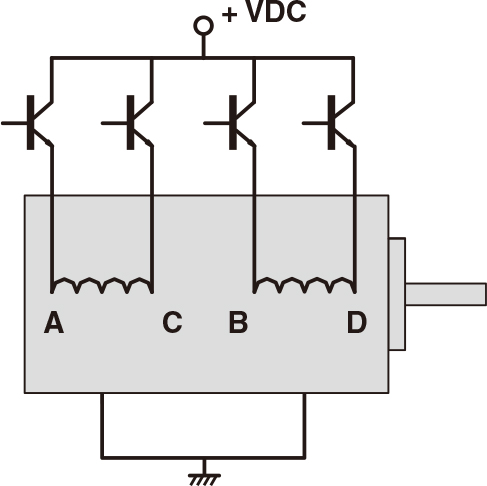
\includegraphics[height=5cm]{step-motor-2-phase-with-unipolar-driver.jpg}
      \caption{2相(单极性)步进电机}
      \label{fig:unipolar}
    \end{minipage}
\end{figure}


\section{步进电机转矩和速度特性}

步进电机的转动距离正比于施加到驱动器上的脉冲信号数(脉冲数)。

步进电机转动(电机出力轴转动角度$\theta$)和脉冲数A的关系如下所示:

\begin{equation}
    \theta=\theta_{s} \times A
\end{equation}

其中$\theta_{s}$为基本步距角,单位是度。

步进电机以一个固定的步距角转动,就像时钟内的秒针。这个角度称为基本步距角。一种标准电机是基本步距角为1.8度的两相步进电机。

步进电机的转速与施加到驱动器上的脉冲信号频率成比例关系。

电机的转速$\mathrm{N}$[r/min] 与脉冲频率$\mathrm{f}$[Hz] 的关系如下(整步模式):

\begin{equation}
    \mathrm{N}=\frac{\theta_{\mathrm{s}}}{360} \times \mathrm{f} \times 60
\end{equation}

步进电机的重要特征之一是高力矩、小体积。如图~\ref{fig:step-servo-motord}。

\begin{figure}[htbp]
    \centering
    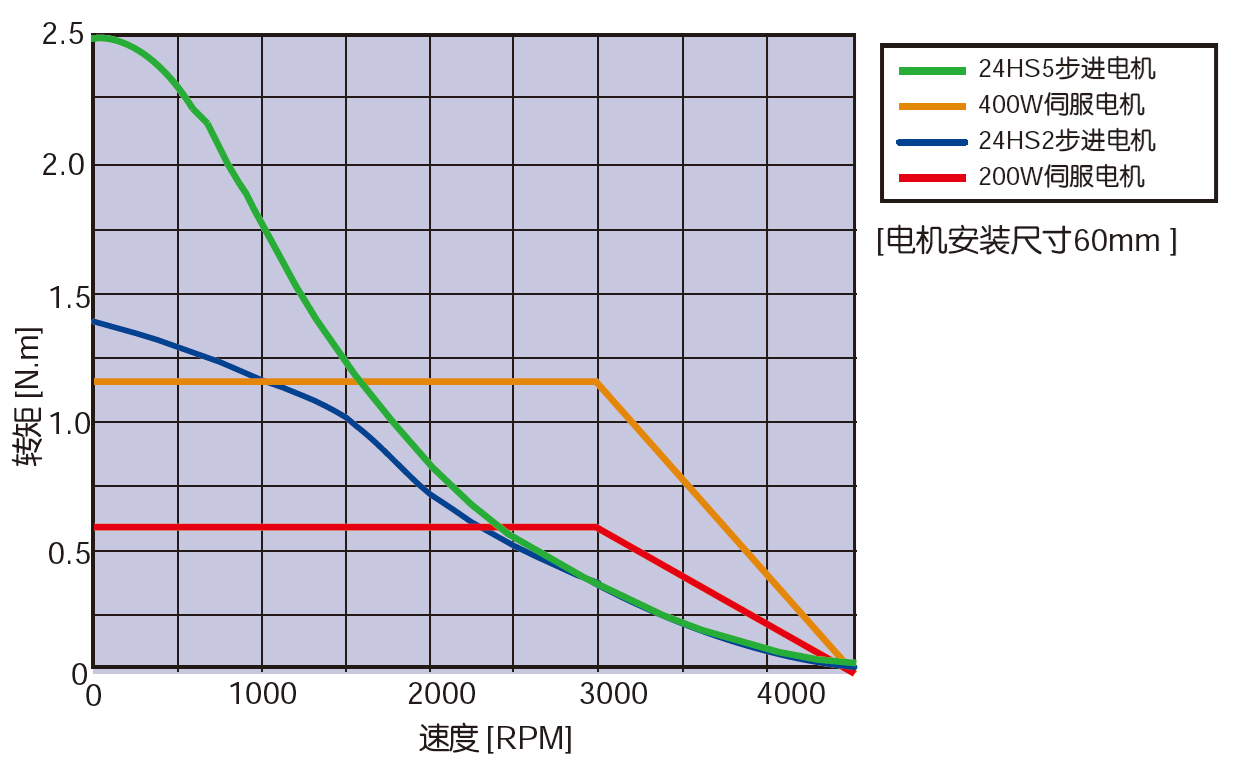
\includegraphics[width=\columnwidth]{step-servo-motord.jpg}
    \caption{相同尺寸下的伺服电机与步进电机的速度力矩特性比较}
    \label{fig:step-servo-motord}
\end{figure}

这些特征使得电机具有优秀的加速和响应,使得这些电机非常适合那些需要频繁启动和停止的应用中。

绕组通电时步进电机具有全部的保持力矩。这就意味着步进电机可以在不使用机械刹车的情况下保持在停止位置。

步进电机的输出力矩随转速升高而下降,且在较高转速时会急剧下降,所以其最高工作转速一般在300~600RPM。

静力矩是选择步进电机的主要参数之一,在判断需要多大的静力矩时要保证步进电机的输出转矩大于负载所需的转矩,这样才能保证整个系统的正常运转,而负载可分为惯性负载和摩擦负载两种。单一的惯性负载和单一的摩擦负载是不存在的。直接启动时两种负载均要考虑,加速启动时主要考虑惯性负载,恒速运行时只要考虑摩擦负载。在计算整个机械系统的负载转矩时,电机的矩频特性能满足机械负载并有一定的余量保证其可靠运行(步进电机的安全系数一般选择1.3~2)。在实际工作过程中,各种频率下的负载转矩必须在矩频特性曲线的范围内,一般来说,静力矩越大的电机,输出转矩也越大,承受负载能力越强。

速度-力矩曲线(图~\ref{fig:step-motor-force})是步进电机输出特性的重要表现形式。

\begin{figure}[htbp]
    \centering
    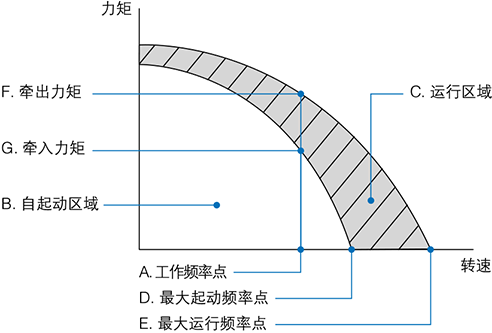
\includegraphics[width=\columnwidth]{step-motor-force.png}
    \caption{速度-力矩曲线}
    \label{fig:step-motor-force}
\end{figure}

A. 工作频率点 电机在某一点的转速值。

速率:

n = q * Hz / (360 * D)

n: 转/秒

Hz: 频率值

D: 驱动电路细分值

q: 步距角

步距角1.8°的步进电机,在 1/2 细分驱动方式下 (即每步 0.9°) 、 工作频率 500Hz 时的转速为1.25r/s.

B. 自启动区域: 步进电机可以直接启动和停止的区域。

C. 连续运行区域: 在该区域内,电机无法直接启动或停止。电机在该区域内运行必须先经过自启动区域,然后经 过加速达到该工作区域运行。同理,电机在该区域内也无法直接制动,否则容易造成电机失步, 必须先经过减速到达自启动区域内再制动。

D. 最高启动频率: 空载情况下,已励磁电机直接启动而不丢步的最高脉冲频率。

E. 最高运行频率: 空载情况下,已励磁电机运行而不丢步的最高脉冲频率。

F. 启动力矩/牵入力矩: 已励磁电机能以某一固定的频率启动和同步运行而不丢步的最大转矩。

G. 运行力矩/牵出力矩: 在规定的驱动条件下,按照给定脉冲频率,可加给已驱动电机转轴上而不是电机丢步的最大转矩。

\section{单极性驱动和双极性驱动的区别}

双极步进电机(Bipolar motors\footnote{\url{https://en.wikipedia.org/wiki/Stepper_motor}})每相只有一个绕组。为了使磁极反向,需要使绕组中的电流反向,因此驱动电路必须更复杂,通常采用H桥配置(但是有几种现成的驱动器芯片可以使之成为一个简单的事情)。每相有两个引线,没有公用的。

两线圈双极步进步进电机的典型驱动模式为:A + B + A- B-。即以正电流驱动线圈A,然后从线圈A中去除电流。然后以正电流驱动线圈B,然后从线圈B中去除电流。然后用负电流驱动线圈A(通过切换导线,例如用H桥翻转极性),然后从线圈A去除电流。然后用负电流驱动线圈B(与线圈A的翻转极性相同);循环完成并重新开始。

由于更好地利用了绕组,因此它们比同等重量的单极步进电机更强大。这是由于绕组占用的物理空间。单极电机在相同的空间中具有两倍的导线数量,但在任何时间点仅使用一半的导线,因此效率为50\%(或大约70\%的可用扭矩输出)。尽管双极步进电机的驱动更加复杂,但丰富的驱动芯片简化了实际使用时的复杂度。

单极性 (unipolar) 和双极性 (bipolar) 是步进电机最常采用的两种驱动电路。单极性驱动电路使用四颗晶体管来驱动步进电机的两组相位,电机定子绕线结构如图~\ref{fig:step-motor-unibipolar}所示包含两组带有中间抽头的线圈(AC线圈的中间抽头为O,BD线圈的中间抽头为M),整个电机共有六条线与外界连接。AC端不能同时通电(BD端同理),否则磁极上的两个线圈产生的磁通相互抵消,只产生线圈的铜耗。因为它其实只有两个相位(AC绕组为一相,BD绕组为一相),准确的说法应是两相六线式步进电机。

\begin{figure}[htbp]
    \centering
    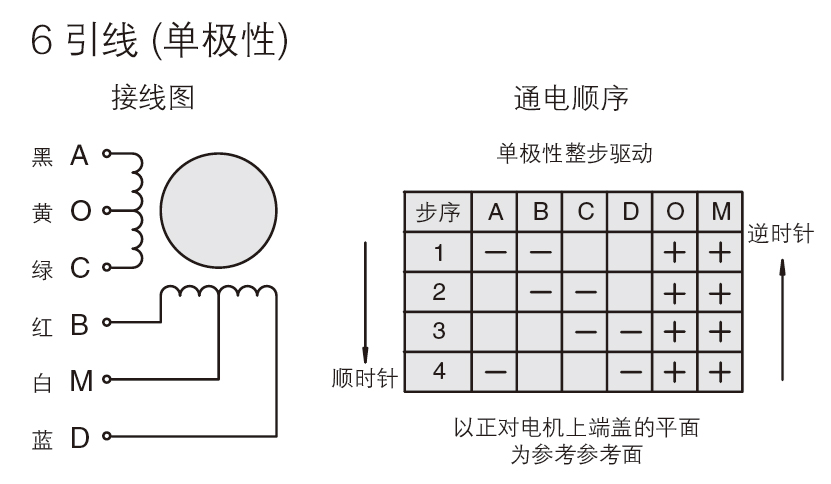
\includegraphics[width=\columnwidth]{step-motor-unibipolar.jpg}
    \caption{单极性驱动电路}
    \label{fig:step-motor-unibipolar}
\end{figure}

双极性步进电机的驱动电路则如图~\ref{fig:step-motor-unibipolar-2}所示,它使用八颗晶体管来驱动两组相位。定子磁极的线圈为单线圈绕组,通过切换线圈AC和线圈BD的的电流方向来切换磁极的正反方向。步进电机的发展初期由于受到晶体管半导体原件的成本影响,单极性电机由于其控制电路使用的晶体管数量少而得到一定范围的应用,但是随着上世纪五六十年代半导体材料的高速发展,晶体管成本大大降低,双极性电机凭借着性能上的优势使其使用量急剧增加。

\begin{figure}[htbp]
    \centering
    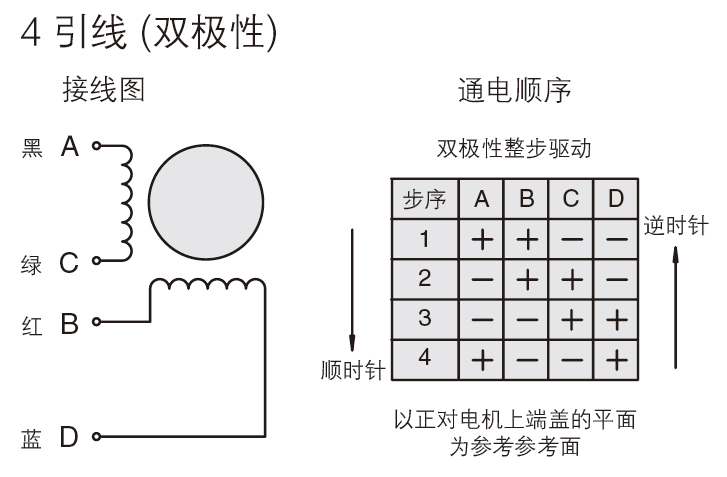
\includegraphics[width=\columnwidth]{step-motor-unibipolar-2.jpg}
    \caption{双极性驱动电路}
    \label{fig:step-motor-unibipolar-2}
\end{figure}

图~\ref{fig:step-motor-unibipolar-3}所示的是单极性与双极性两种绕线方式,导线线径相同时,单极方式的线圈绕组匝数为N,电阻为R,双极方式的线圈绕组匝数为2N,线圈电阻则为2R。

\begin{figure}[htbp]
    \centering
    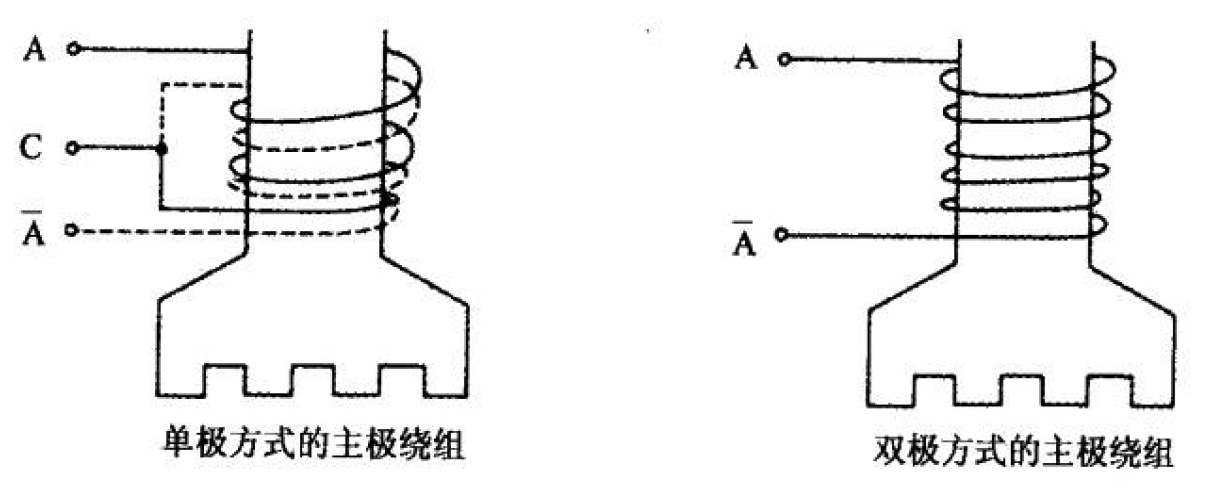
\includegraphics[width=\columnwidth]{step-motor-unibipolar-3.jpg}
    \caption{单极性与双极性绕组}
    \label{fig:step-motor-unibipolar-3}
\end{figure}

表~\ref{tab:step-motor-unibipolar}所示恒压驱动电路在低速时,单极与双极驱动工作效率的对比。电流与线圈匝数的乘积称为安匝数,与转矩成正比,如果两者转速相同,输出功率与安匝数有比例关系。同样,双极性电流为V/2R,匝数也为2N,乘积的结果与单极性同为VN/R。输入恒压驱动的情形,单极性与双极性比较,如表~\ref{tab:step-motor-unibipolar}所示,电流只有单极性的二分之一,低速时的效率为单极性的2倍。

\begin{table}[htbp]
    \centering
    \begin{tabular}{lll}
     & 单极性 & 双极性 \\
    安匝数 & $U_{1}=V \times \frac{N}{R}$ & $U_{2}=V \times \frac{2N}{2R}=V \times \frac{N}{R}$\\
    输入功率 & $W_{1}=\frac{\mathrm{V}^{2}}{R}$ & $\mathrm{W}_{2}=(\frac{\mathrm{V}}{2 \mathrm{R}} )^{2} \times  2 \mathrm{R}=\frac{\mathrm{V}^{2}}{2 \mathrm{R}} $ \\
    效率 & $\eta = \frac{U_{1}}{W_{1}} = \frac{N}{V}$ & $\eta = \frac{U_{2}}{W_{2}} = \frac{2N}{V}$
    \end{tabular}
    \caption{单极驱动与双极驱动效率对比 注:V为所加电压;R为电机线圈电阻;N为单极匝数}
    \label{tab:step-motor-unibipolar}
\end{table}

所以小型化或低速应用时,有大转矩需求,应使用双极性电机及驱动。高速应用的情况下,因为双极性电机匝数多,电感变大,反电势增大,使高速时电流减少,从而降低转矩,所以需要注意与单极性的转矩比较。

图~\ref{fig:step-motor-unibipolar-4}为单极性步进电机与双极性步进电机的特性曲线,均采用同一恒流驱动方式。一般低速大转矩的负载应用使用双极性驱动,而高速驱动应用以单极性驱动较为合适。

\begin{figure}[htbp]
    \centering
    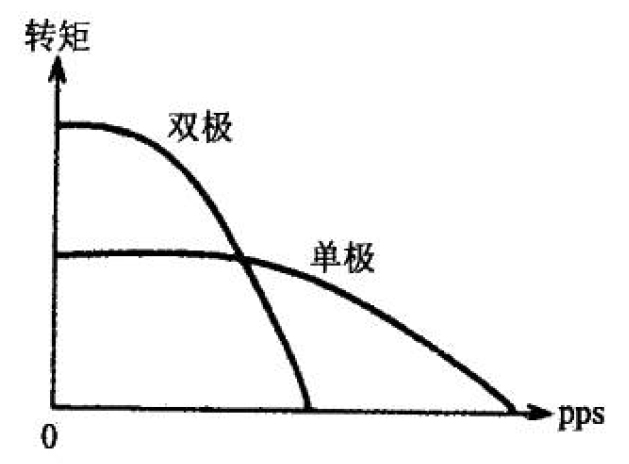
\includegraphics[width=0.5\columnwidth]{step-motor-unibipolar-4.jpg}
    \caption{单极驱动与双极驱动的矩频曲线对比}
    \label{fig:step-motor-unibipolar-4}
\end{figure}

\section{步进电机驱动}

斩波驱动电路(Chopper drive circuits)称为受控电流驱动器,因为它们在每个绕组中产生受控电流,而不是施加恒定电压。斩波器驱动电路最常用于双绕组双极步进电机,两个绕组被独立驱动以提供特定的步进电机转矩CW或CCW。在每个绕组上,将“电源”电压作为方波电压施加到绕组上。例如8 kHz。绕组电感使电流平滑,该电流达到根据方波占空比的水平。相对于绕组回路,双极性电源(+和-)电压通常提供给控制器。

如图~\ref{fig:Phase-current}

\begin{figure}[htbp]
    \centering
    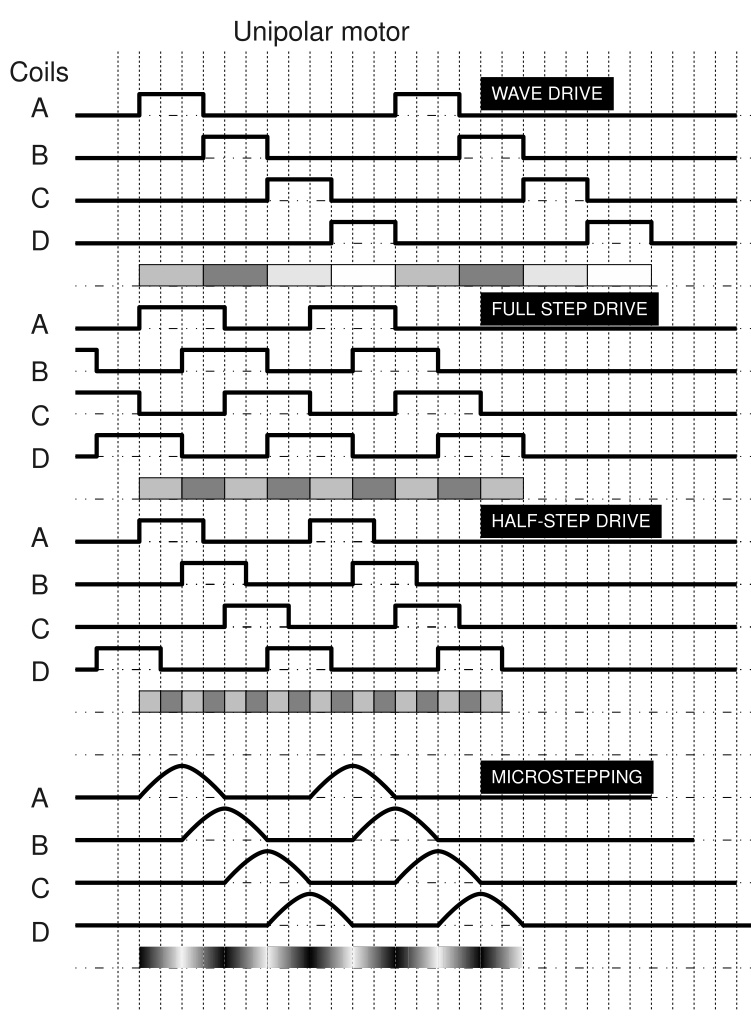
\includegraphics[width=\columnwidth]{Drive.png}
    \caption{Phase current waveforms}
    \label{fig:Phase-current}
\end{figure}

\section{步进电机驱动DRV8825}

DRV8825用于双极步进电机控制。微步步进电机驱动器提供更高的精度以及步进电机平稳的旋转。

\begin{figure}[htbp]
    \centering
    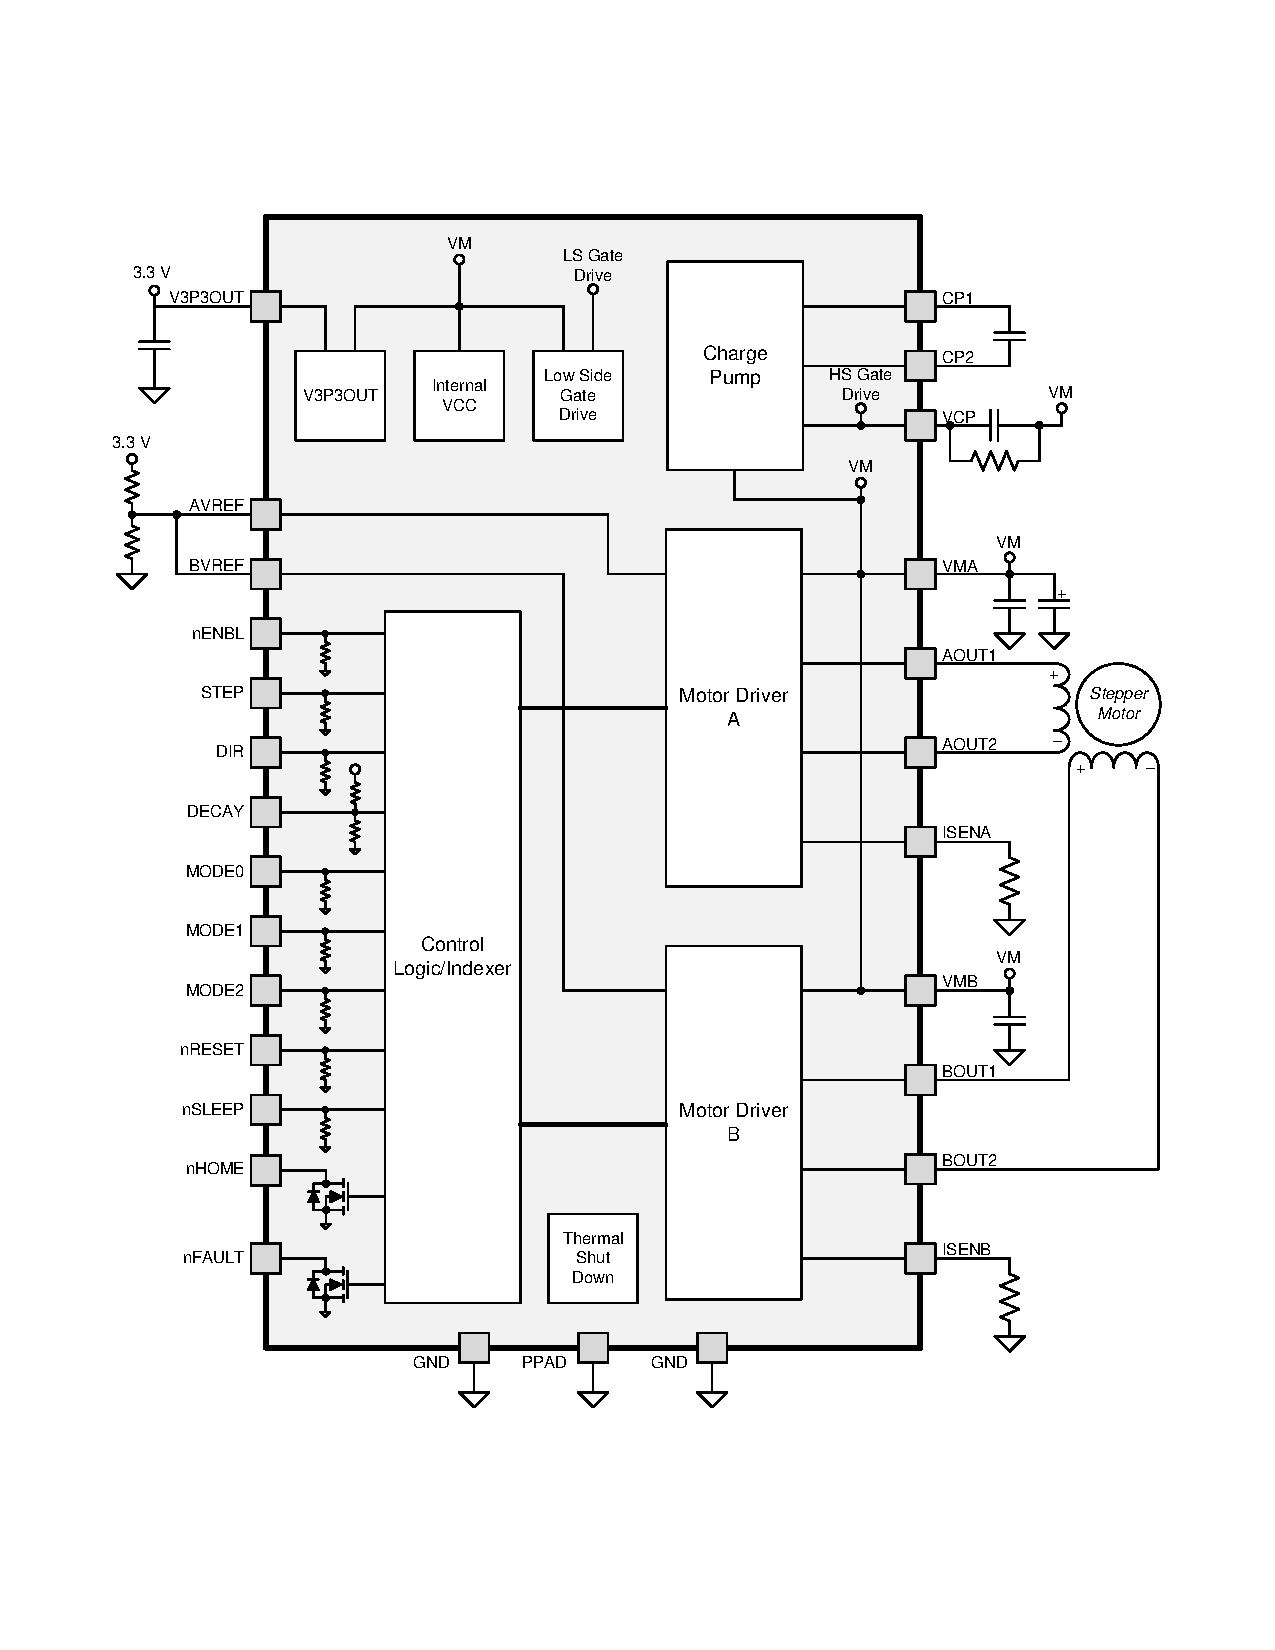
\includegraphics[width=\columnwidth]{DRV8825-Function-Block.pdf}
    \caption{DRV8825功能框图}
    \label{fig:DRV8825-Function-Block}
\end{figure}

配置DRV8825的第一步需要所需的转速和微步级别。

\begin{figure}[htbp]
    \centering
    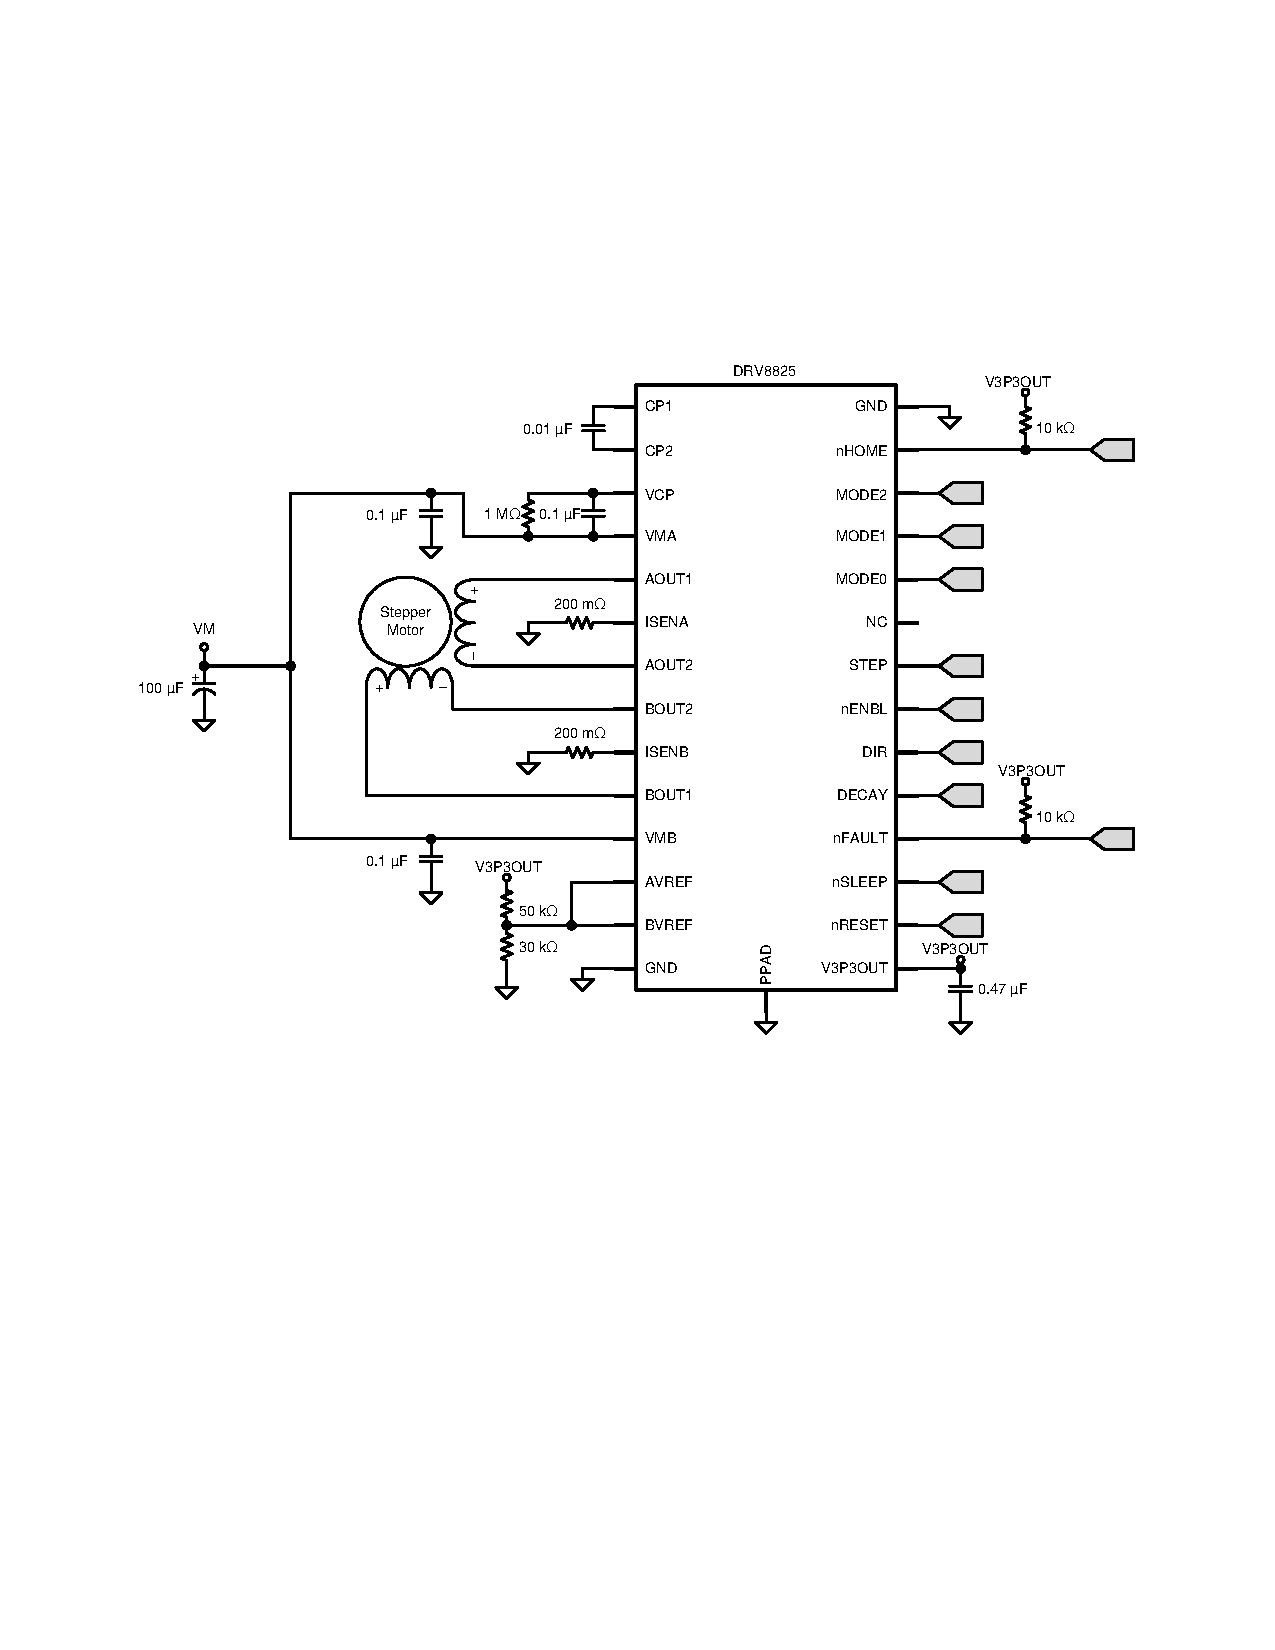
\includegraphics[width=\columnwidth]{DRV8825-Typical-Application.pdf}
    \caption{DRV8825典型应用}
    \label{fig:DRV8825-Typical-Application}
\end{figure}


\begin{figure}[htbp]
    \centering
    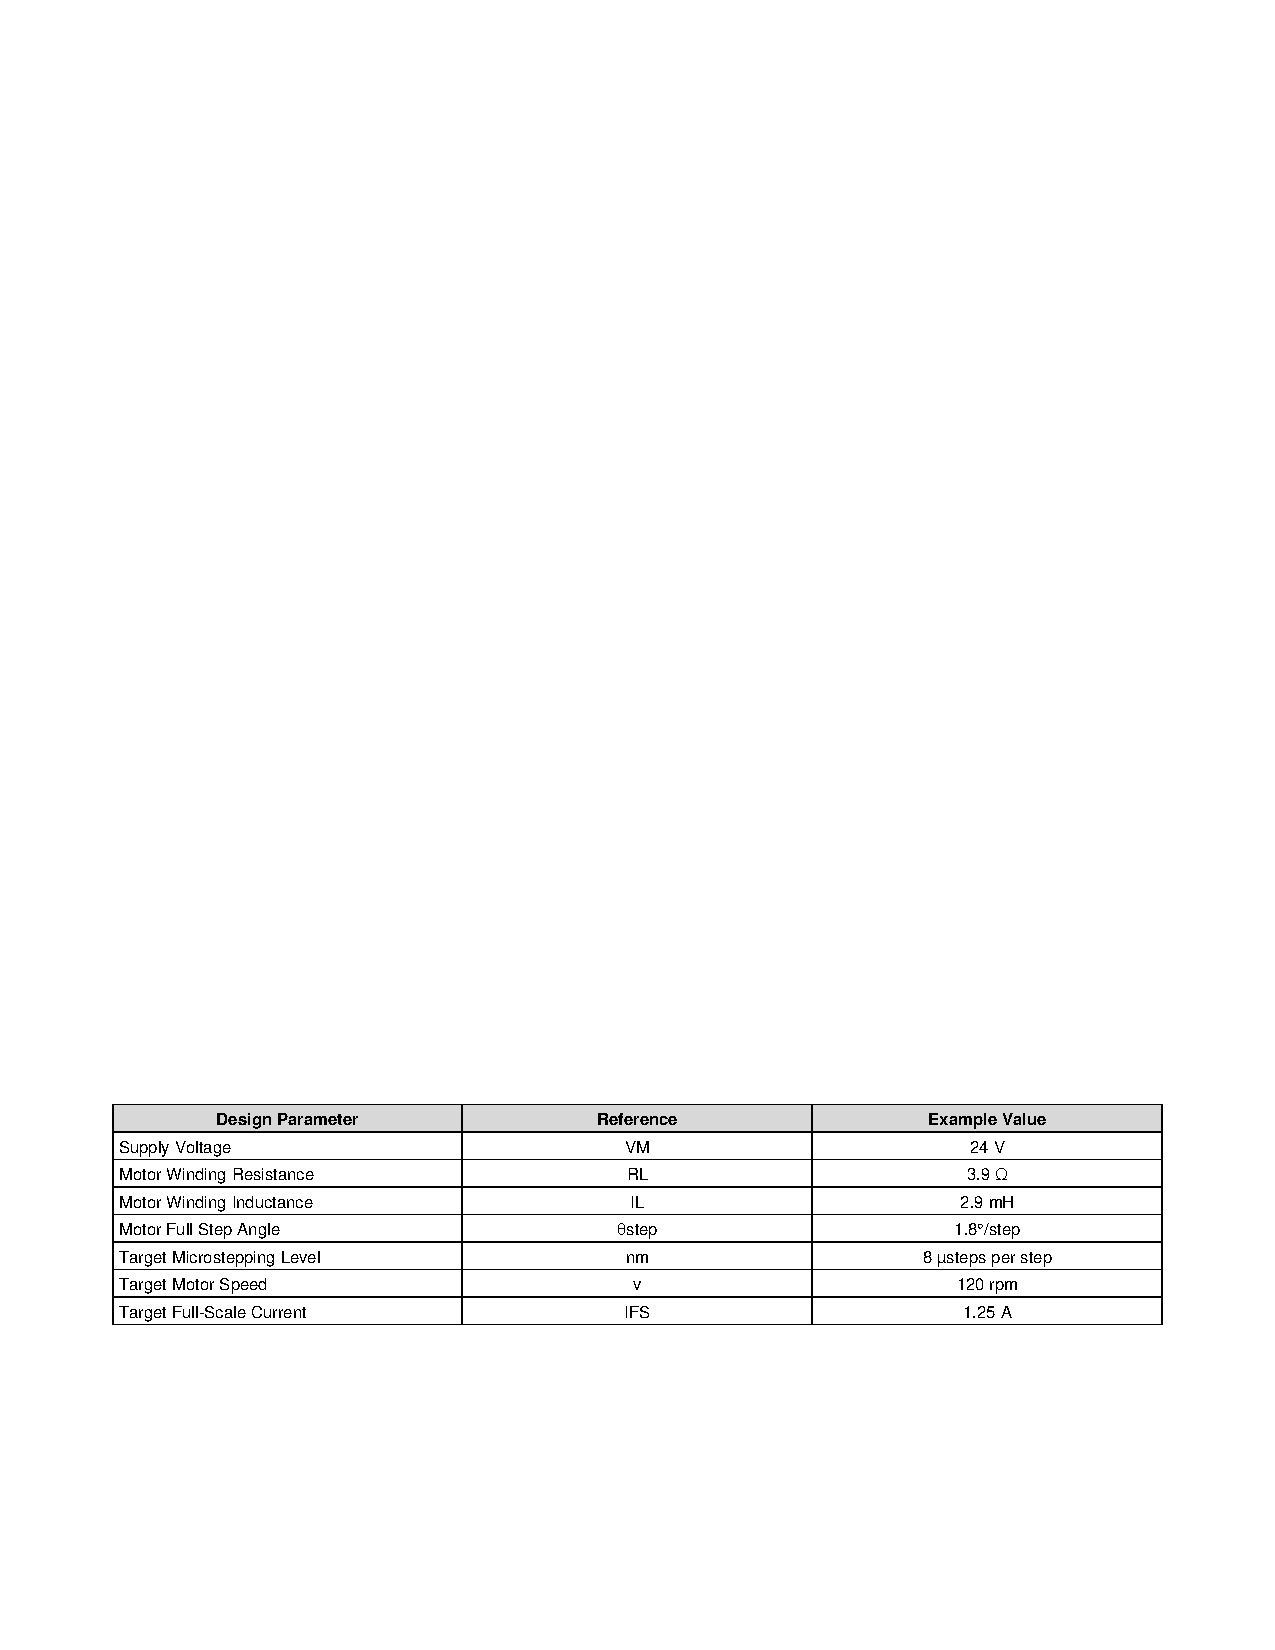
\includegraphics[width=\columnwidth]{DRV8825-Design-Requirements.pdf}
    \caption{DRV8825设计要求}
    \label{fig:DRV8825-Design-Requirements}
\end{figure}

如果需要恒定转速,则将频率为$f_step$的方波施加到STEP引脚。

如果步进电机的目标速度过高,步进电机可能不会旋转。 确保步进电机可以支持目标速度或通过加速以使步进电机达到最高速度。

对于所需的步进电机速度(v),微步级别($n_m$)和步进电机全步距角($\theta_{\text {step }}$,一整步对应的角度),

\begin{equation}
    \begin{aligned}
    &f_{\text {step }(\mu \text { steps } / \text { second })=} \frac{v\left(\frac{\text { rotations }}{\text { minute }}\right) \times 360\left(\frac{\circ}{\text { rotation }}\right) \times n_{\mathrm{m}}\left(\frac{\mu \text { steps }}{\text { step }}\right)}{60\left(\frac{\text { seconds }}{\text { minute }}\right) \times \theta_{\text {step }}\left(\frac{^{\circ}}{\text { step }}\right)}\\
    &f_{\text {step }(\mu \text { steps } / \text { second })=} \frac{120\left(\frac{\text { rotations }}{\text { minute }}\right) \times 360\left(\frac{^{\circ}}{\text { rotation }}\right) \times 8\left(\frac{\mu \text { steps }}{\text { step }}\right)}{60\left(\frac{\text { seconds }}{\text { minute }}\right) \times 1.8\left(\frac{\circ}{\text { step }}\right)}
    \end{aligned}
\end{equation}

DRV8825微步步进级别由MODE引脚设置,如表~\ref{tab:DRV8825-microstep-settings}所示。

\begin{table}[htbp]
    \centering
    \begin{tabular}{llll}
    \hline
    M0   & M1   & M2   & Microstep resolution \\ \hline
    Low  & Low  & Low  & Full step            \\ \hline
    High & Low  & Low  & 1/2 step             \\ \hline
    Low  & High & Low  & 1/4 step             \\ \hline
    High & High & Low  & 1/8 step             \\ \hline
    Low  & Low  & High & 1/16 step            \\ \hline
    High & Low  & High & 1/32 step            \\ \hline
    Low  & High & High & 1/32 step            \\ \hline
    High & High & High & 1/32 step            \\ \hline
    \end{tabular}
    \caption{DRV8825 microstep settings}
    \label{tab:DRV8825-microstep-settings}
\end{table}

较高的微步步进级别将意味着步进电机运动更平稳且噪声较小,但会增加开关损耗,并且需要较高的$f_step$才能达到相同的步进电机速度。

在步进电机中,设定的满量程电流($I_{FS}$ full-scale current)是通过任一绕组驱动的最大电流。 该数量取决于xVREF模拟电压和检测电阻值($R_{\text {SENSE}}$)。 

在步进期间,IFS定义为最大电流步进斩波阈值($I_{\text {TRIP}}$ current chopping threshold)。 DRV8825的增益设置为5V。

\begin{equation}
    \operatorname{I_{FS}}(A)=\frac{x \operatorname{VREF}(V)}{A_{v} \times R_{S E N S E}(\Omega)}=\frac{x \operatorname{VREF}(V)}{5 \times R_{S E N S E}(\Omega)}
\end{equation}

参考设计和要求如图~\ref{fig:DRV8825-Typical-Application}和图~\ref{fig:DRV8825-Design-Requirements}

典型模块设计和布局如图~\ref{fig:DRV8825-stepper-motor-driver-carrier-schematic-diagram}和图~\ref{fig:DRV8825-Layout-Example}

\begin{figure}[htbp]
    \centering
    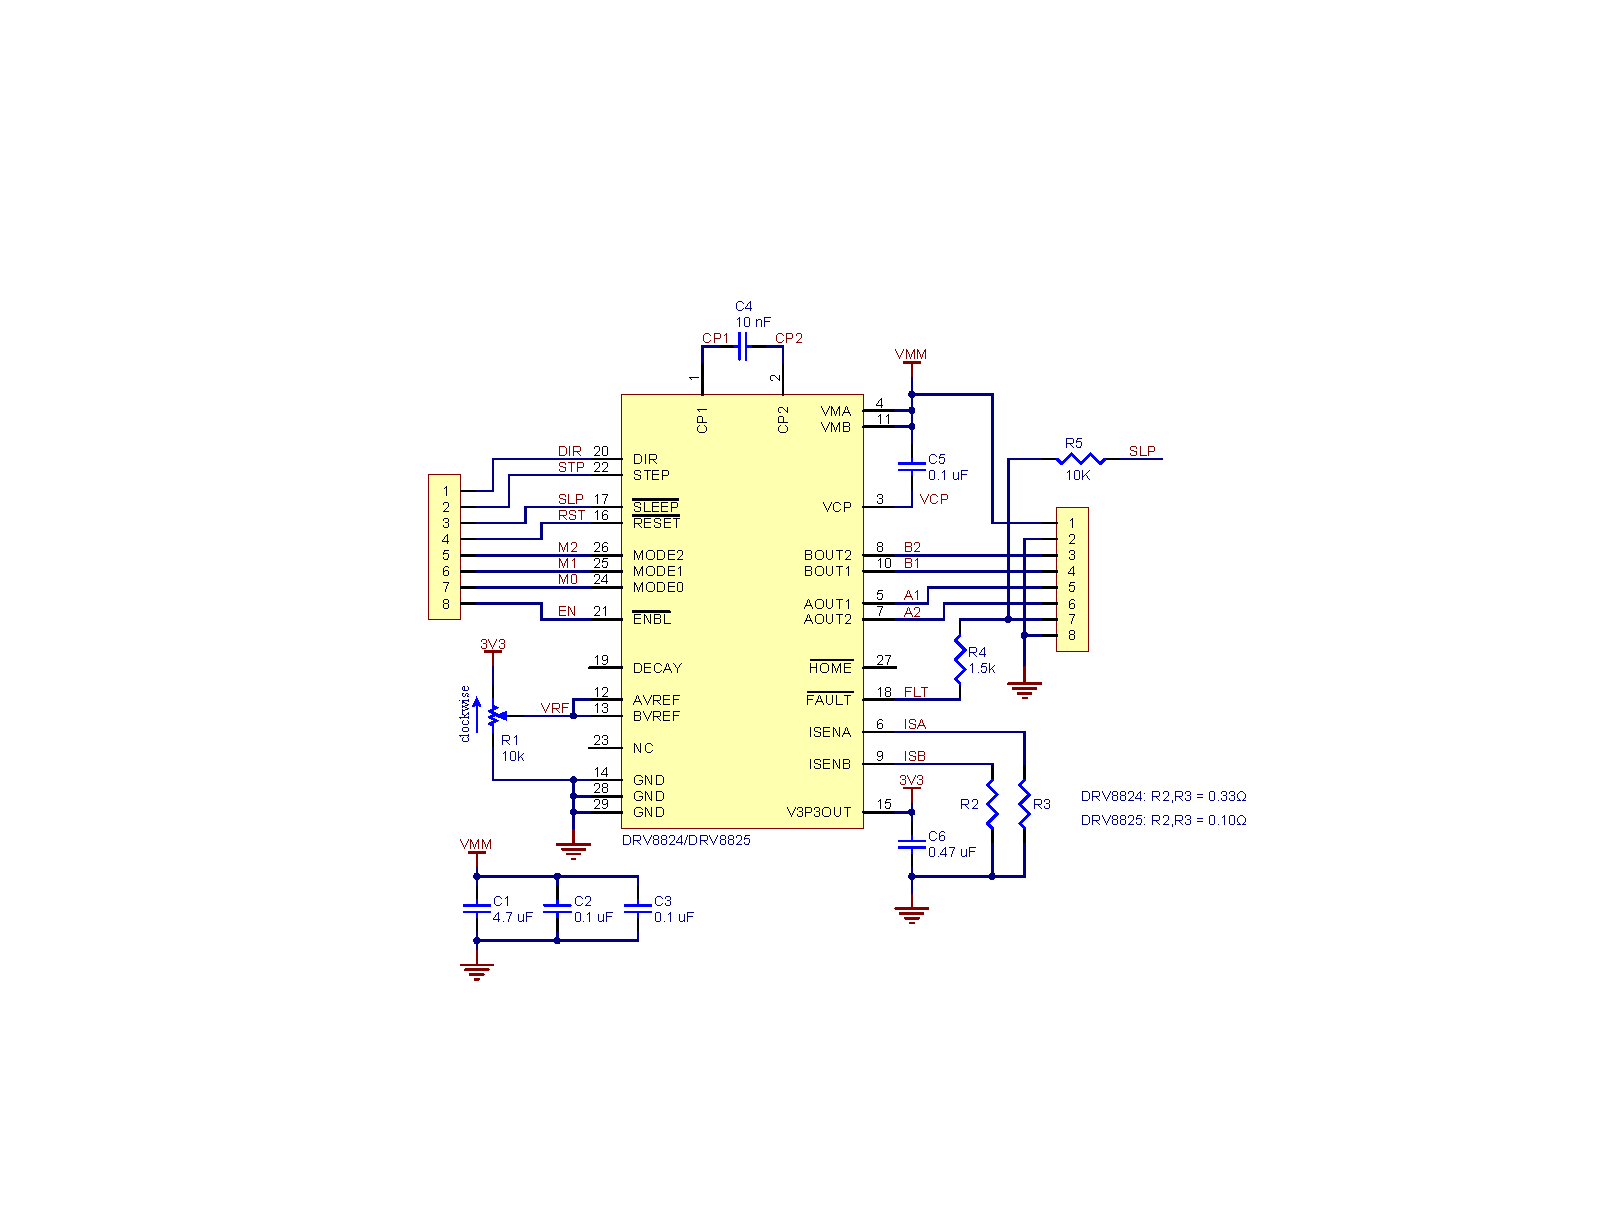
\includegraphics[width=\columnwidth]{drv8824-drv8825-stepper-motor-driver-carrier-schematic-diagram.pdf}
    \caption{DRV8825模块设计 DRV8824/DRV8825 Stepper Motor Driver Carrier}
    \label{fig:DRV8825-stepper-motor-driver-carrier-schematic-diagram}
\end{figure}

\begin{figure}[htbp]
    \centering
    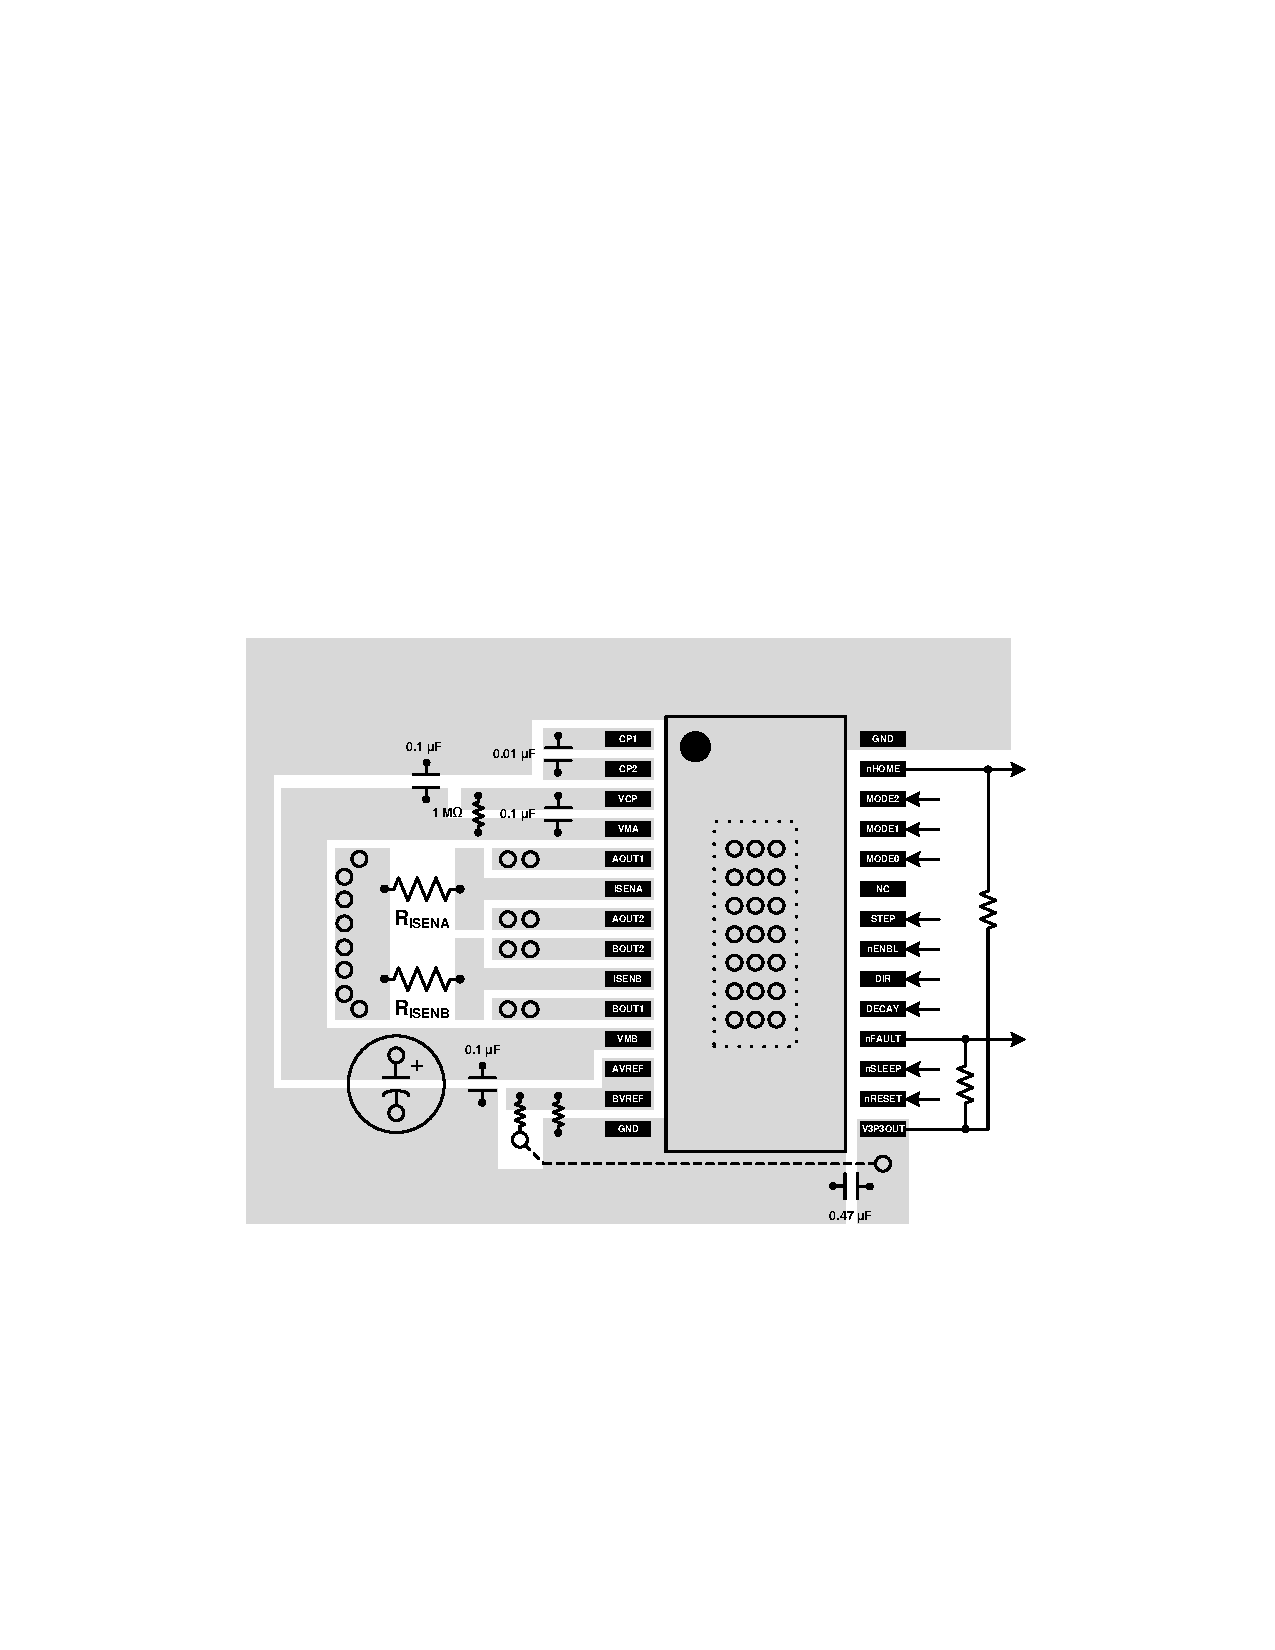
\includegraphics[width=\columnwidth]{DRV8825-Layout-Example.pdf}
    \caption{DRV8825布局参考}
    \label{fig:DRV8825-Layout-Example}
\end{figure}


\section{减速步进电机}

CHS-GM1024-10BY 2相4线直径15BY全金属齿轮减速步进电机 参数如图~\ref{fig:CHS-GM1024-10BY-Specific}所示。

\begin{figure}[htbp]
    \centering
    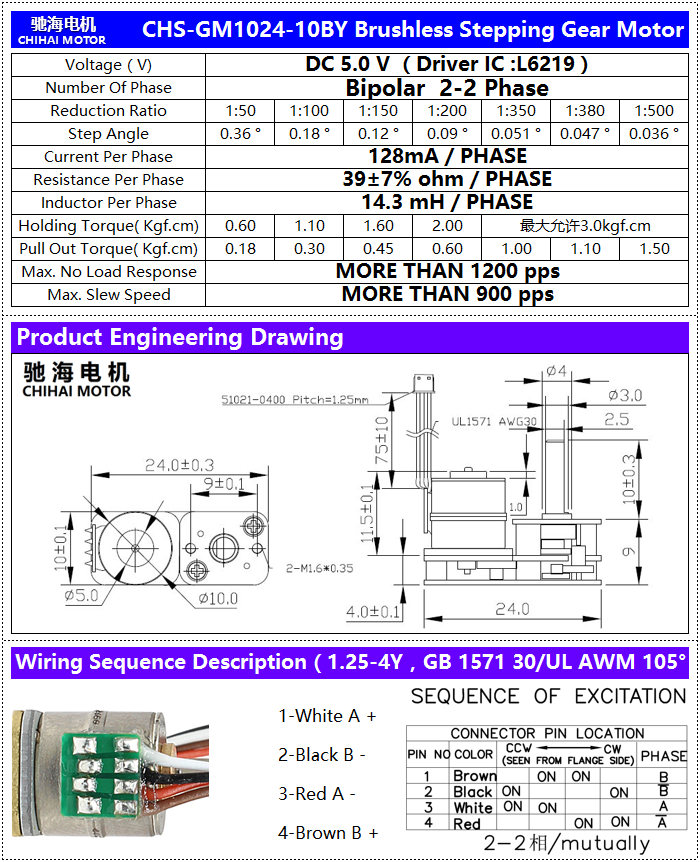
\includegraphics[width=\columnwidth]{CHS-GM1024-10BY-Specific.jpg}
    \caption{CHS-GM1024-10BY参数}
    \label{fig:CHS-GM1024-10BY-Specific}
\end{figure}

\begin{table}[htbp]
    \centering
    \begin{tabular}{ll}
    \hline
    Model                  & CHS-GM1024-10BY   \\ \hline
    Working voltage        & DC 5V             \\ \hline
    Phase                  & 2 phase 4 wire    \\ \hline
    Reduction ratio        & 1:100             \\ \hline
    Step angle             & 0.18°             \\ \hline
    Phase current          & 128mA/phase       \\ \hline
    Phase resistance       & 39±7\%ohm/phase   \\ \hline
    Phase inductance       & 14.3mH/phase      \\ \hline
    Holding torque         & 1.10kgf.cm        \\ \hline
    Pull out torque        & 0.30kgf.cm        \\ \hline
    Max starting frequency & More than 1200pps \\ \hline
    Response frequency     & More than 900pps  \\ \hline
    \end{tabular}
    \caption{CHIHAI MOTOR DC 5V Brushless Motor 2 Phase 4 Wire Stepper Motor Specification}
    \label{tab:CHS-GM1024-10BY-Specific}
\end{table}

\section{电机连接器}

采用的电机原装为Molex 51021-0400 连接器 1.25mm Pitch, PicoBlade 1.25 DIP TYPE SMT TYPE \url{https://www.chinese.molex.com/molex/products/part-detail/crimp_housings/0510210400},为了方便未来批量制作,我们使用对应的插座,如图~\ref{fig:51021-APPLICATION-SPECIFICATION}所示。

\begin{figure}[htbp]
    \centering
    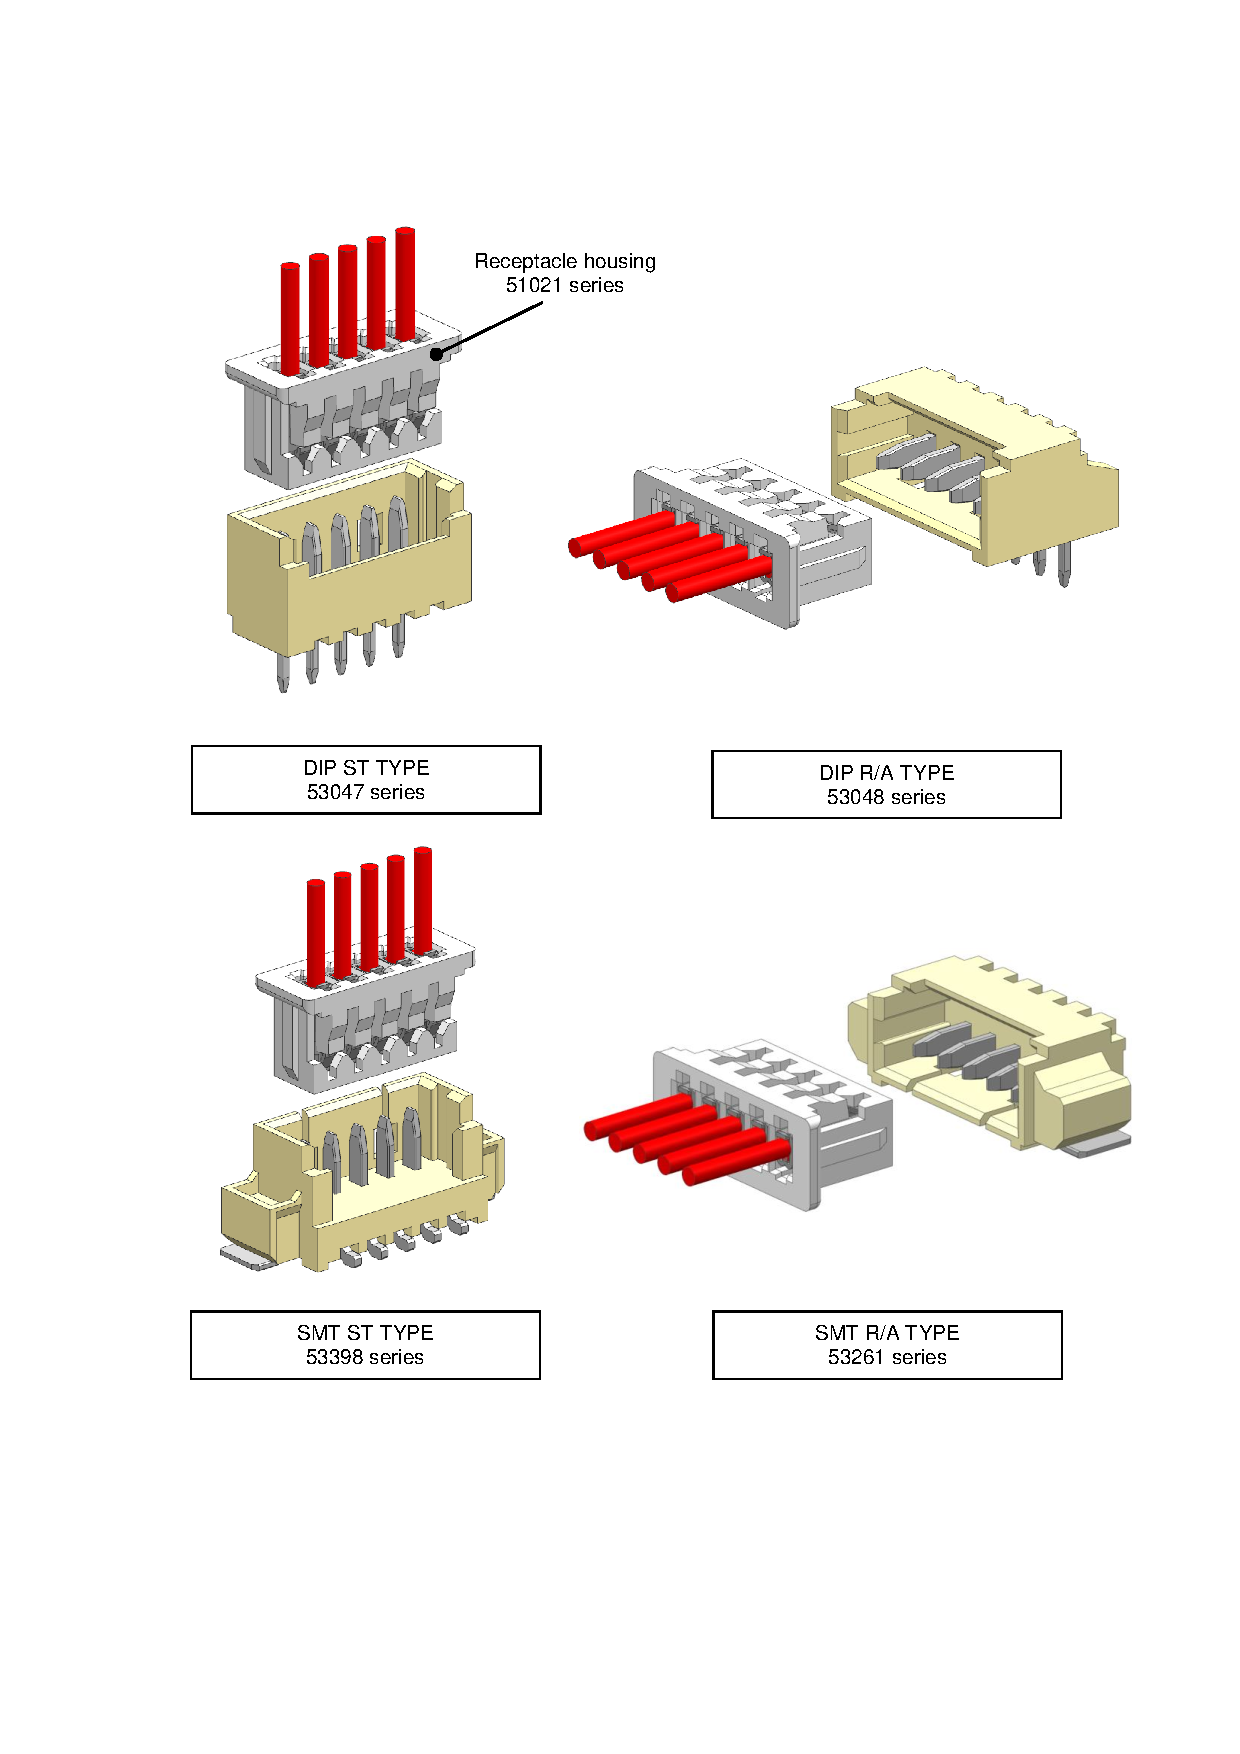
\includegraphics[width=\columnwidth]{51021-APPLICATION-SPECIFICATION.pdf}
    \caption{Molex 51021 连接}
    \label{fig:51021-APPLICATION-SPECIFICATION}
\end{figure}


\section{DRV8825 Arduino 控制程序}

本节设计源文件和历史版本详见\url{https://github.com/TingliangZhang/Misaka-Code}

pps (pulses per second)

Arduino 官方库中默认带有 Stepper Library (\url{https://www.arduino.cc/en/Reference/Stepper}),提供了unipolar or bipolar stepper motors的控制函数。

Stepper(steps, pin1, pin2, pin3, pin4) 函数定义了一个步进电机类的实例

steps: the number of steps in one revolution of your motor. If your motor gives the number of degrees per step, divide that number into 360 to get the number of steps (e.g. 360 / 3.6 gives 100 steps). (int)

问题是Stepper Library针对的是H桥或直连的2/4线简单的步进电机,并非特定的驱动芯片如DRV8825,所以需要其他库。

AccelStepper library for Arduino \url{http://www.airspayce.com/mikem/arduino/AccelStepper/} 则很好的兼容了驱动芯片并且提供加速减速等功能。

AccelStepper Class Reference 参见 \url{http://www.airspayce.com/mikem/arduino/AccelStepper/classAccelStepper.html} 。

函数 AccelStepper (uint8\_t interface=AccelStepper::FULL4WIRE, uint8\_t pin1=2, uint8\_t pin2=3, uint8\_t pin3=4, uint8\_t pin4=5, bool enable=true) 定义了一个步进电机(create a new instance of the AccelStepper class)。

其中interface设置为1,即枚举变量 enum AccelStepper::MotorInterfaceType 取AccelStepper::DRIVER (1),意为连接的是具有Step and Direction pins的步进电机驱动芯片。pin1连接到步进电机驱动Step引脚,低电平到高电平跳变为步进。pin2连接到步进电机驱动Direction引脚,高电平为正向旋转。其他变量留空默认即可。

以下操作函数需要用到使用AccelStepper实例化的名字,定义小车的三个轮子的步进电机分别为Motor1、Motor2、Motor3。

\begin{itemize}
    \item setMaxSpeed
    \item setAcceleration
    \item moveTo
    \item runToPosition
    \item runSpeed
    \item distanceToGo
    \item currentPosition
\end{itemize}


\section{单电机测试}

测试接线图如图~\ref{fig:Arduino-DRV8825}

\begin{figure}[htbp]
    \centering
    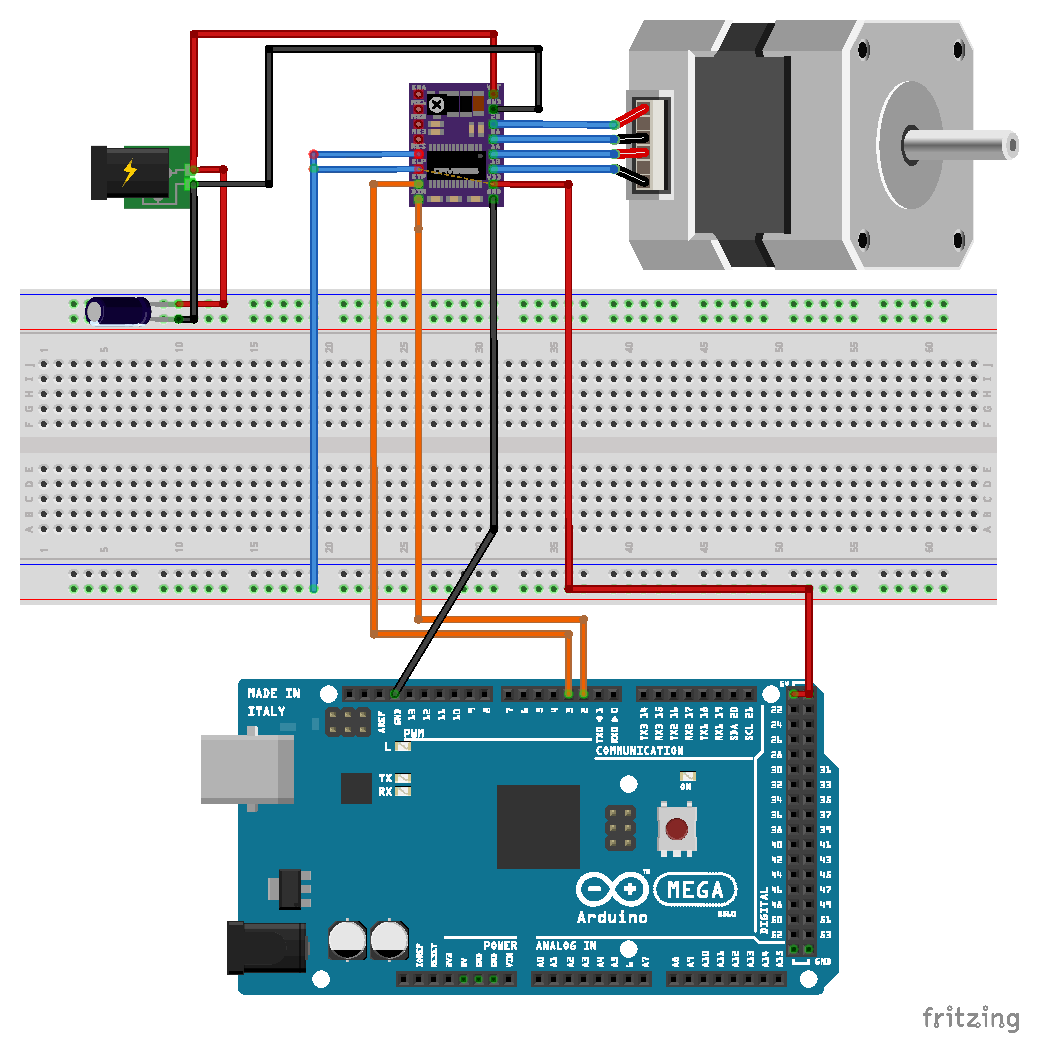
\includegraphics[width=\columnwidth]{Arduino-DRV8825-RE-SAVE.pdf}
    \caption{Arduino-DRV8825接线图}
    \label{fig:Arduino-DRV8825}
\end{figure}


% ERROR!!!!!!!
% xdvipdfmx:fatal: pdf_link_obj(): passed invalid object.
% \begin{figure}[htbp]
%     \centering
%     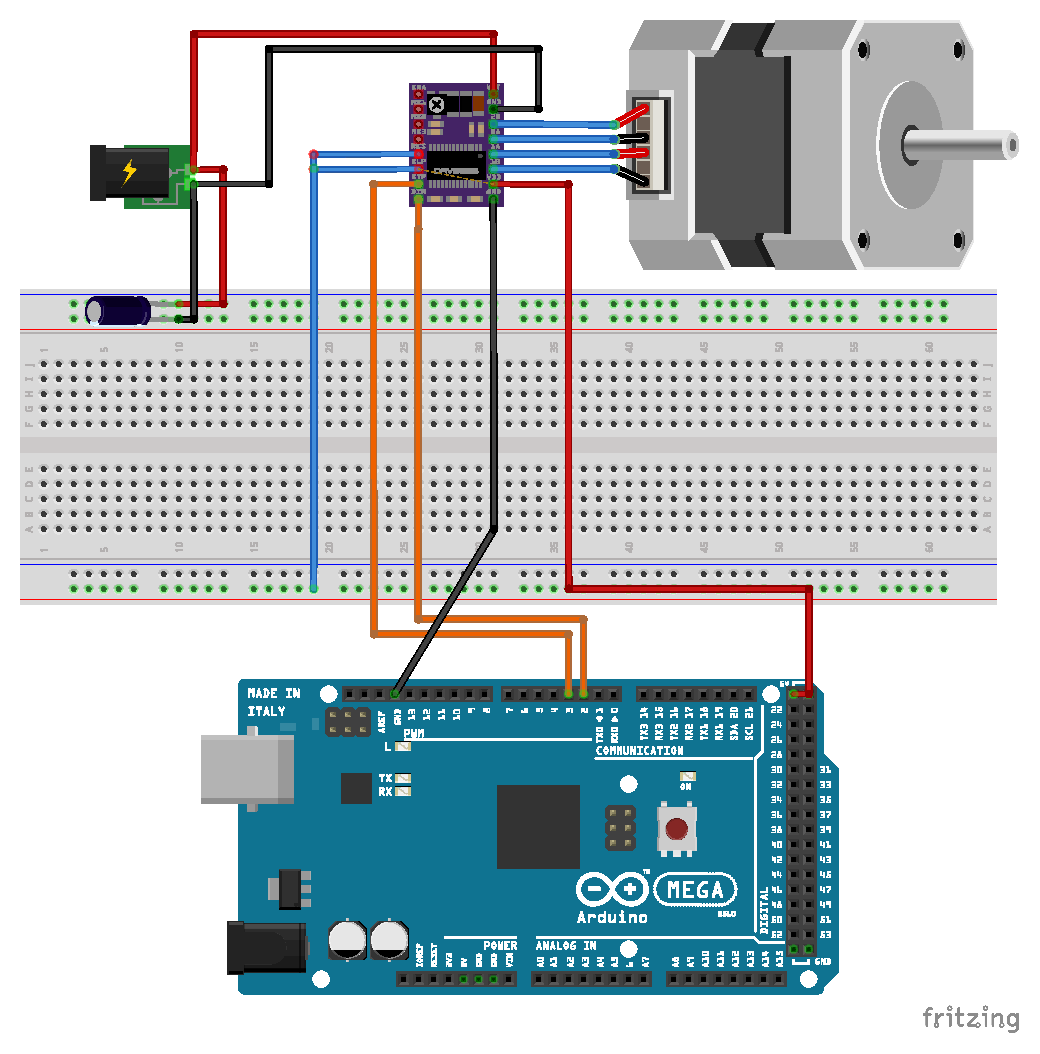
\includegraphics[width=\columnwidth]{Arduino-DRV8825.pdf}
%     \caption{Arduino-DRV8825接线图}
%     \label{fig:Arduino-DRV8825}
% \end{figure}

未接电机时使用如下代码进行加减速测试:

\inputminted[mathescape, linenos, breaklines]{C}{Code/Stepper-3/Stepper-3.ino}

得到波形如图~\ref{fig:AccelStepper-Acceleration-Waveform}、图~\ref{fig:AccelStepper-Acceleration-Waveform-with-motor}、图~\ref{fig:AccelStepper-Acceleration-Spectrogram}。

\begin{figure}[htbp]
    \centering
    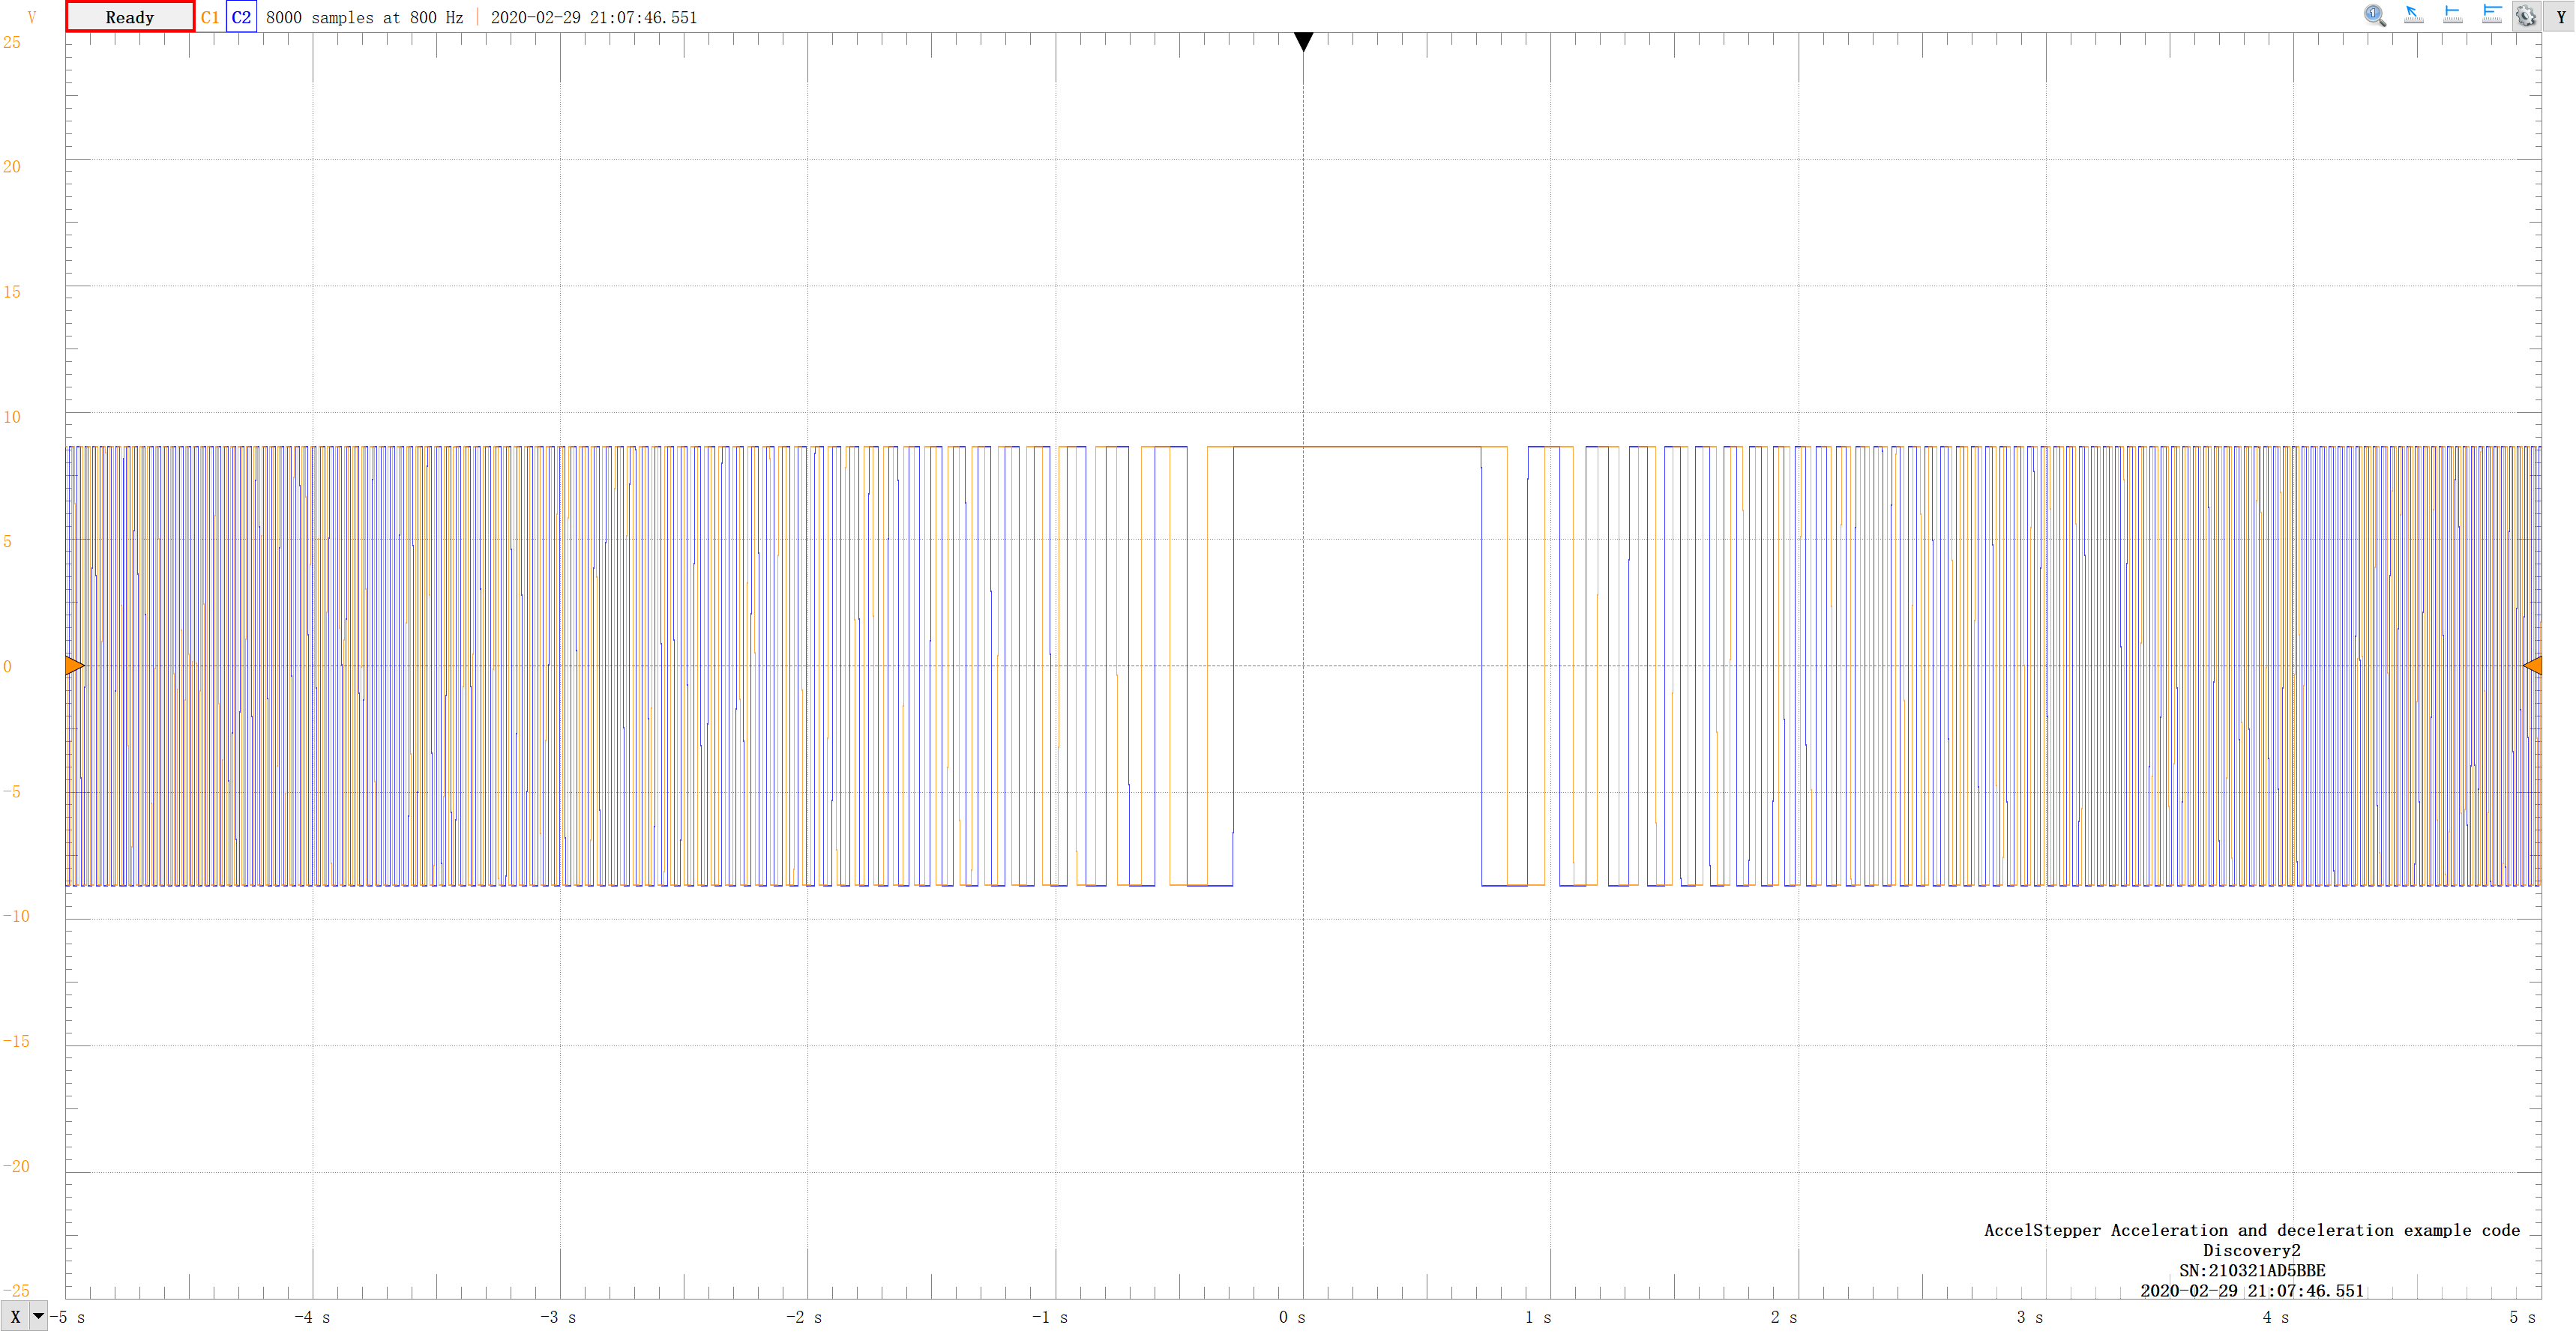
\includegraphics[width=\columnwidth]{AccelStepper-Acceleration-Waveform.png}
    \caption{AccelStepper库加速转动DRV8825未接电机输出驱动波形}
    \label{fig:AccelStepper-Acceleration-Waveform}
\end{figure}

\begin{figure}[htbp]
    \centering
    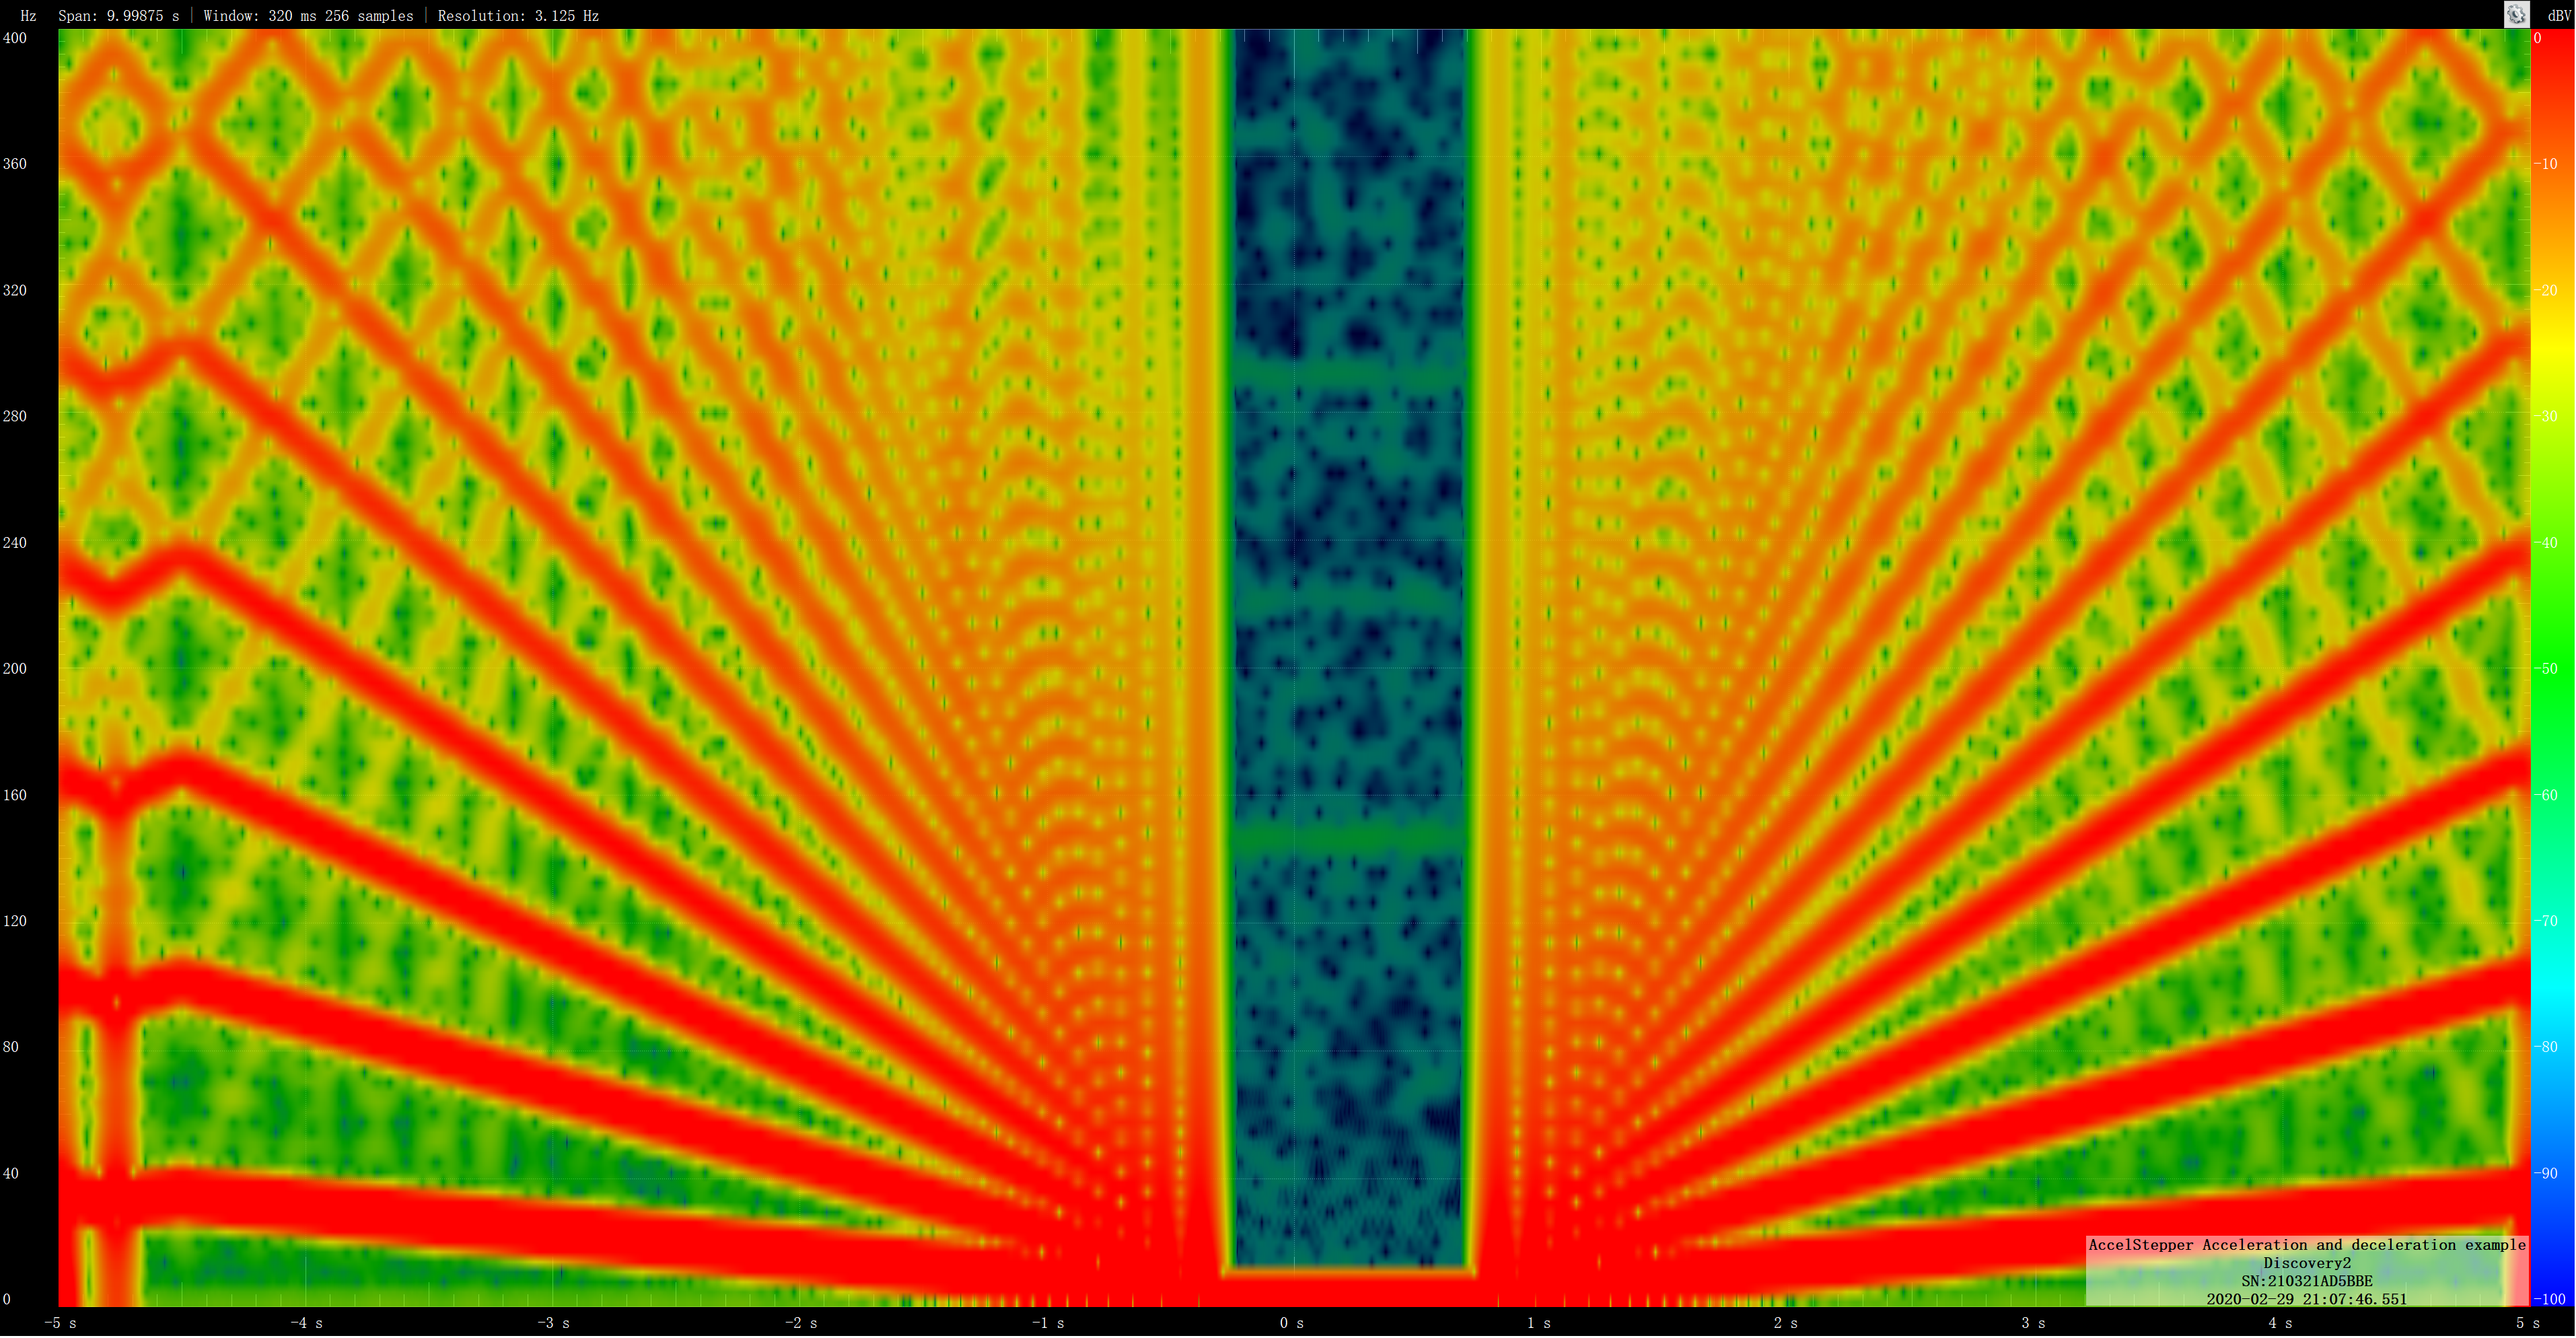
\includegraphics[width=\columnwidth]{AccelStepper-Acceleration-Spectrogram.png}
    \caption{AccelStepper库加速转动DRV8825未接电机驱动输出频谱图}
    \label{fig:AccelStepper-Acceleration-Spectrogram}
\end{figure}

\begin{figure}[htbp]
    \centering
    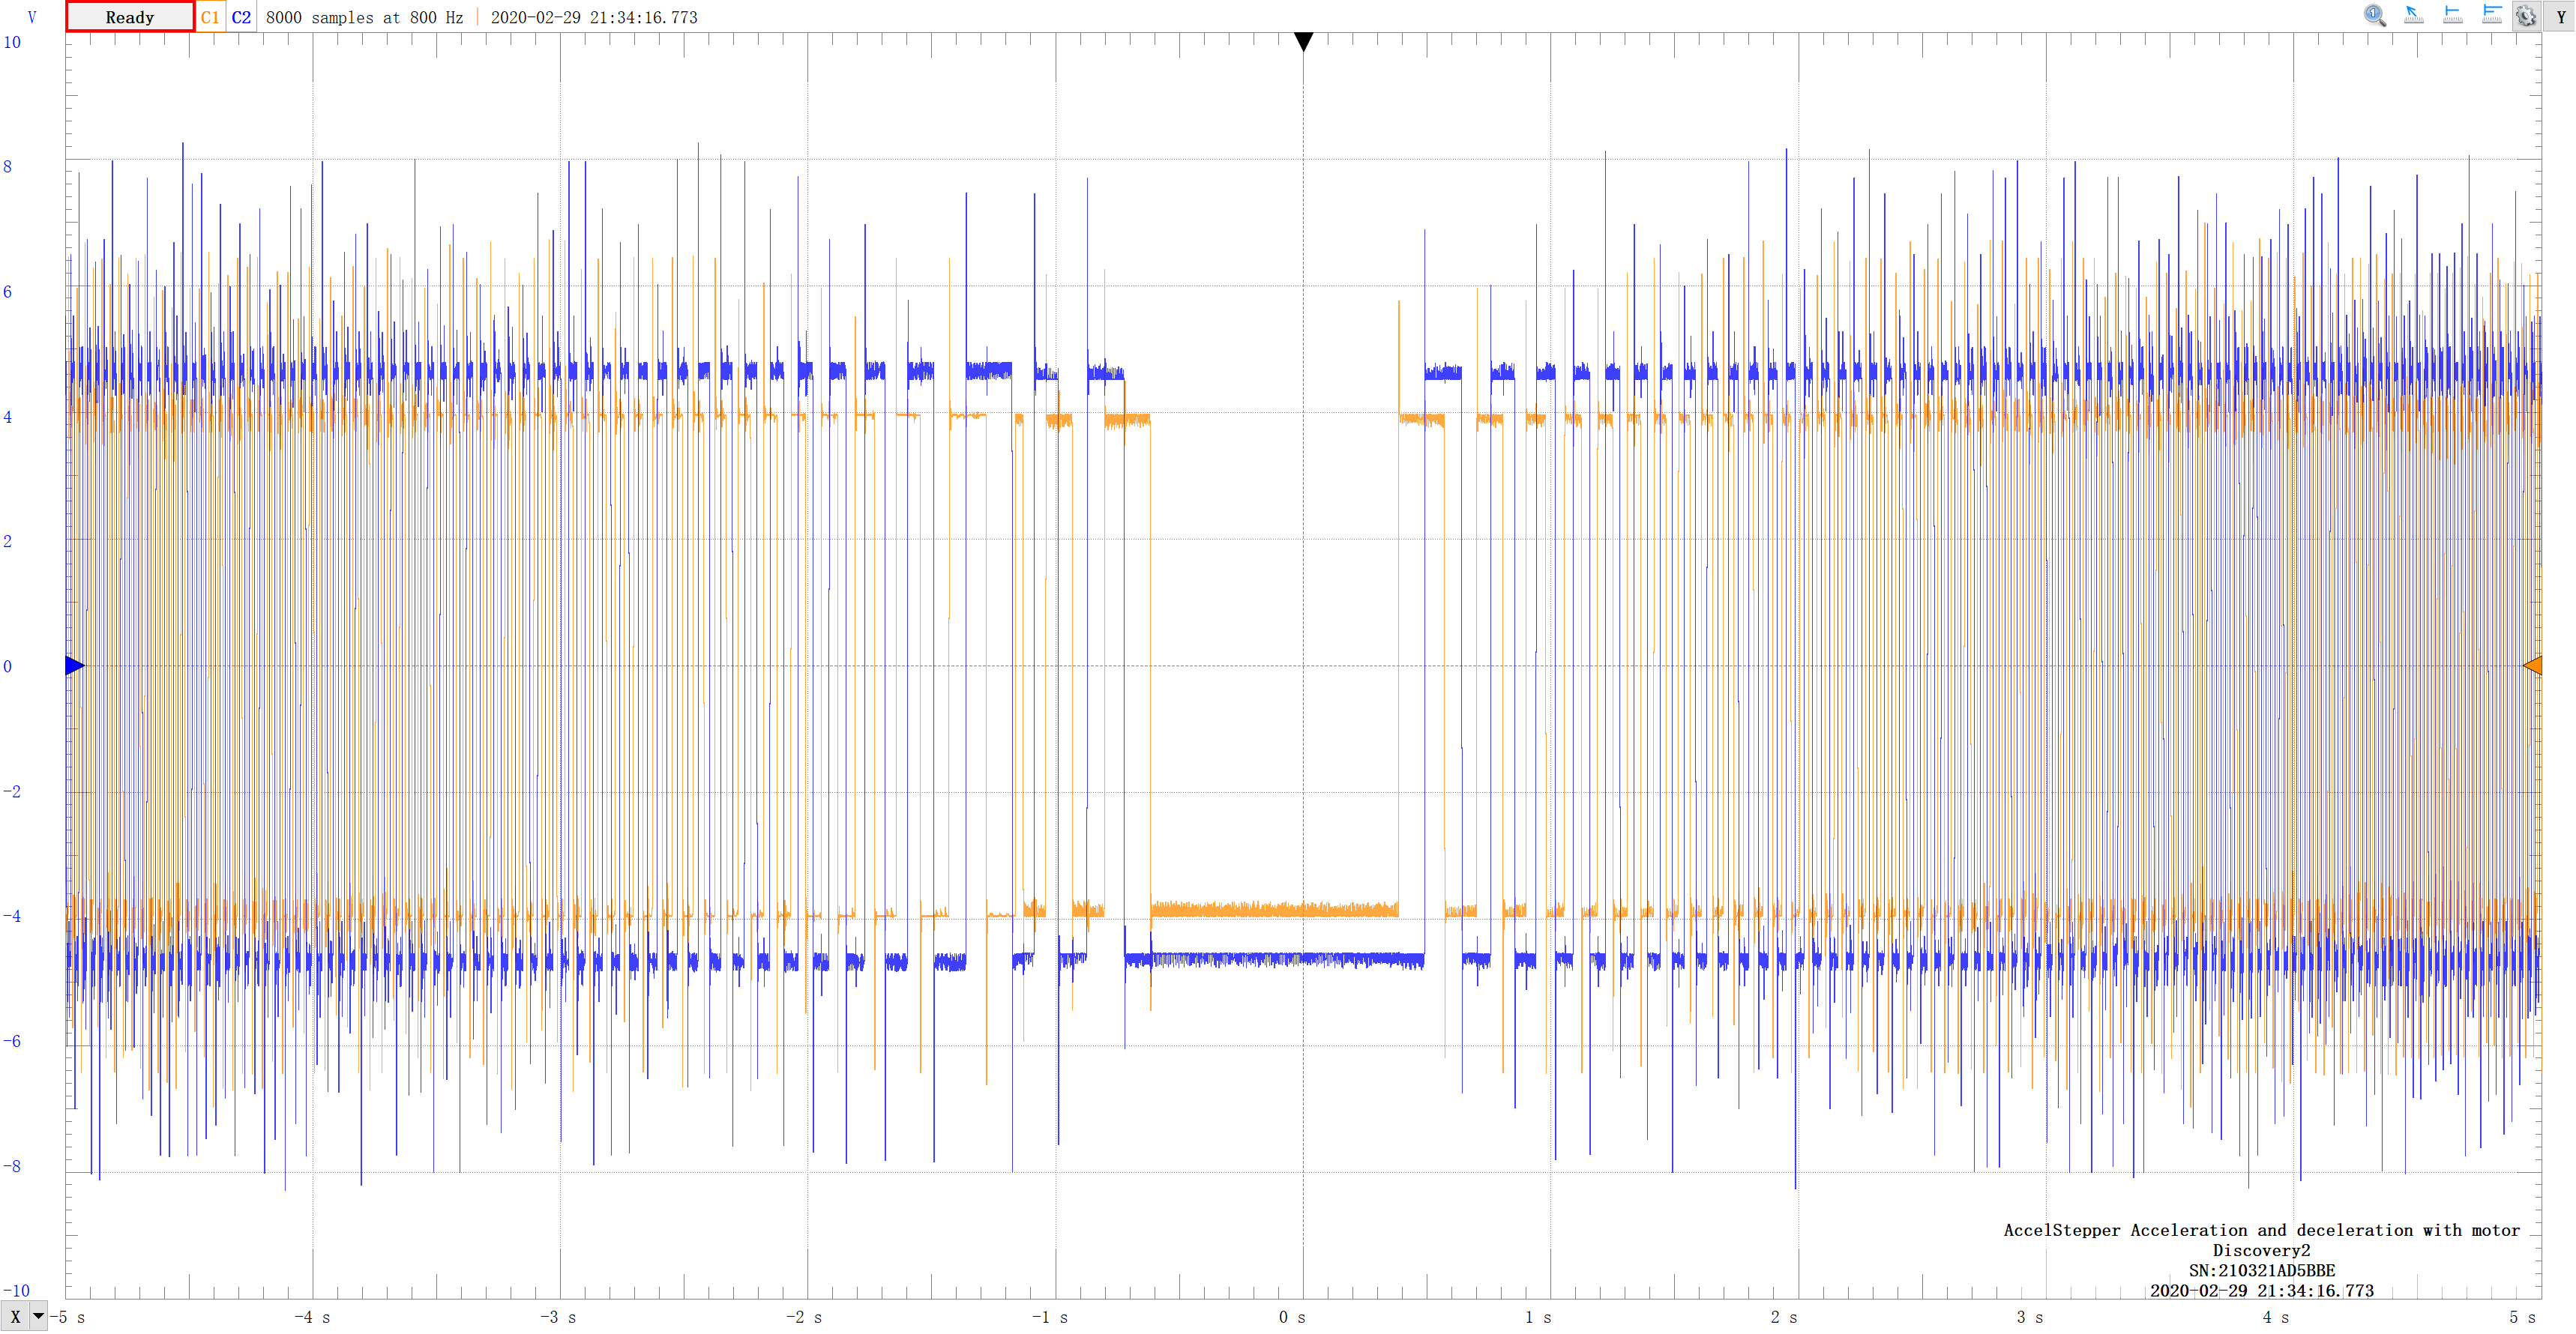
\includegraphics[width=\columnwidth]{AccelStepper-Acceleration-Waveform-with-motor.png}
    \caption{AccelStepper库加速转动DRV8825接电机输出驱动波形}
    \label{fig:AccelStepper-Acceleration-Waveform-with-motor}
\end{figure}

接电机时使用如下代码进行以一定加速度加速到恒定速度测试:

\inputminted[mathescape, linenos, breaklines]{C}{Code/Stepper-3/Stepper-3.ino}

得到波形如图~\ref{fig:AccelStepper-Constant-Speed-Waveform-with-motor}和图~\ref{fig:AccelStepper-Constant-Speed-Waveform-with-motor-Scaled}。

\begin{figure}[htbp]
    \centering
    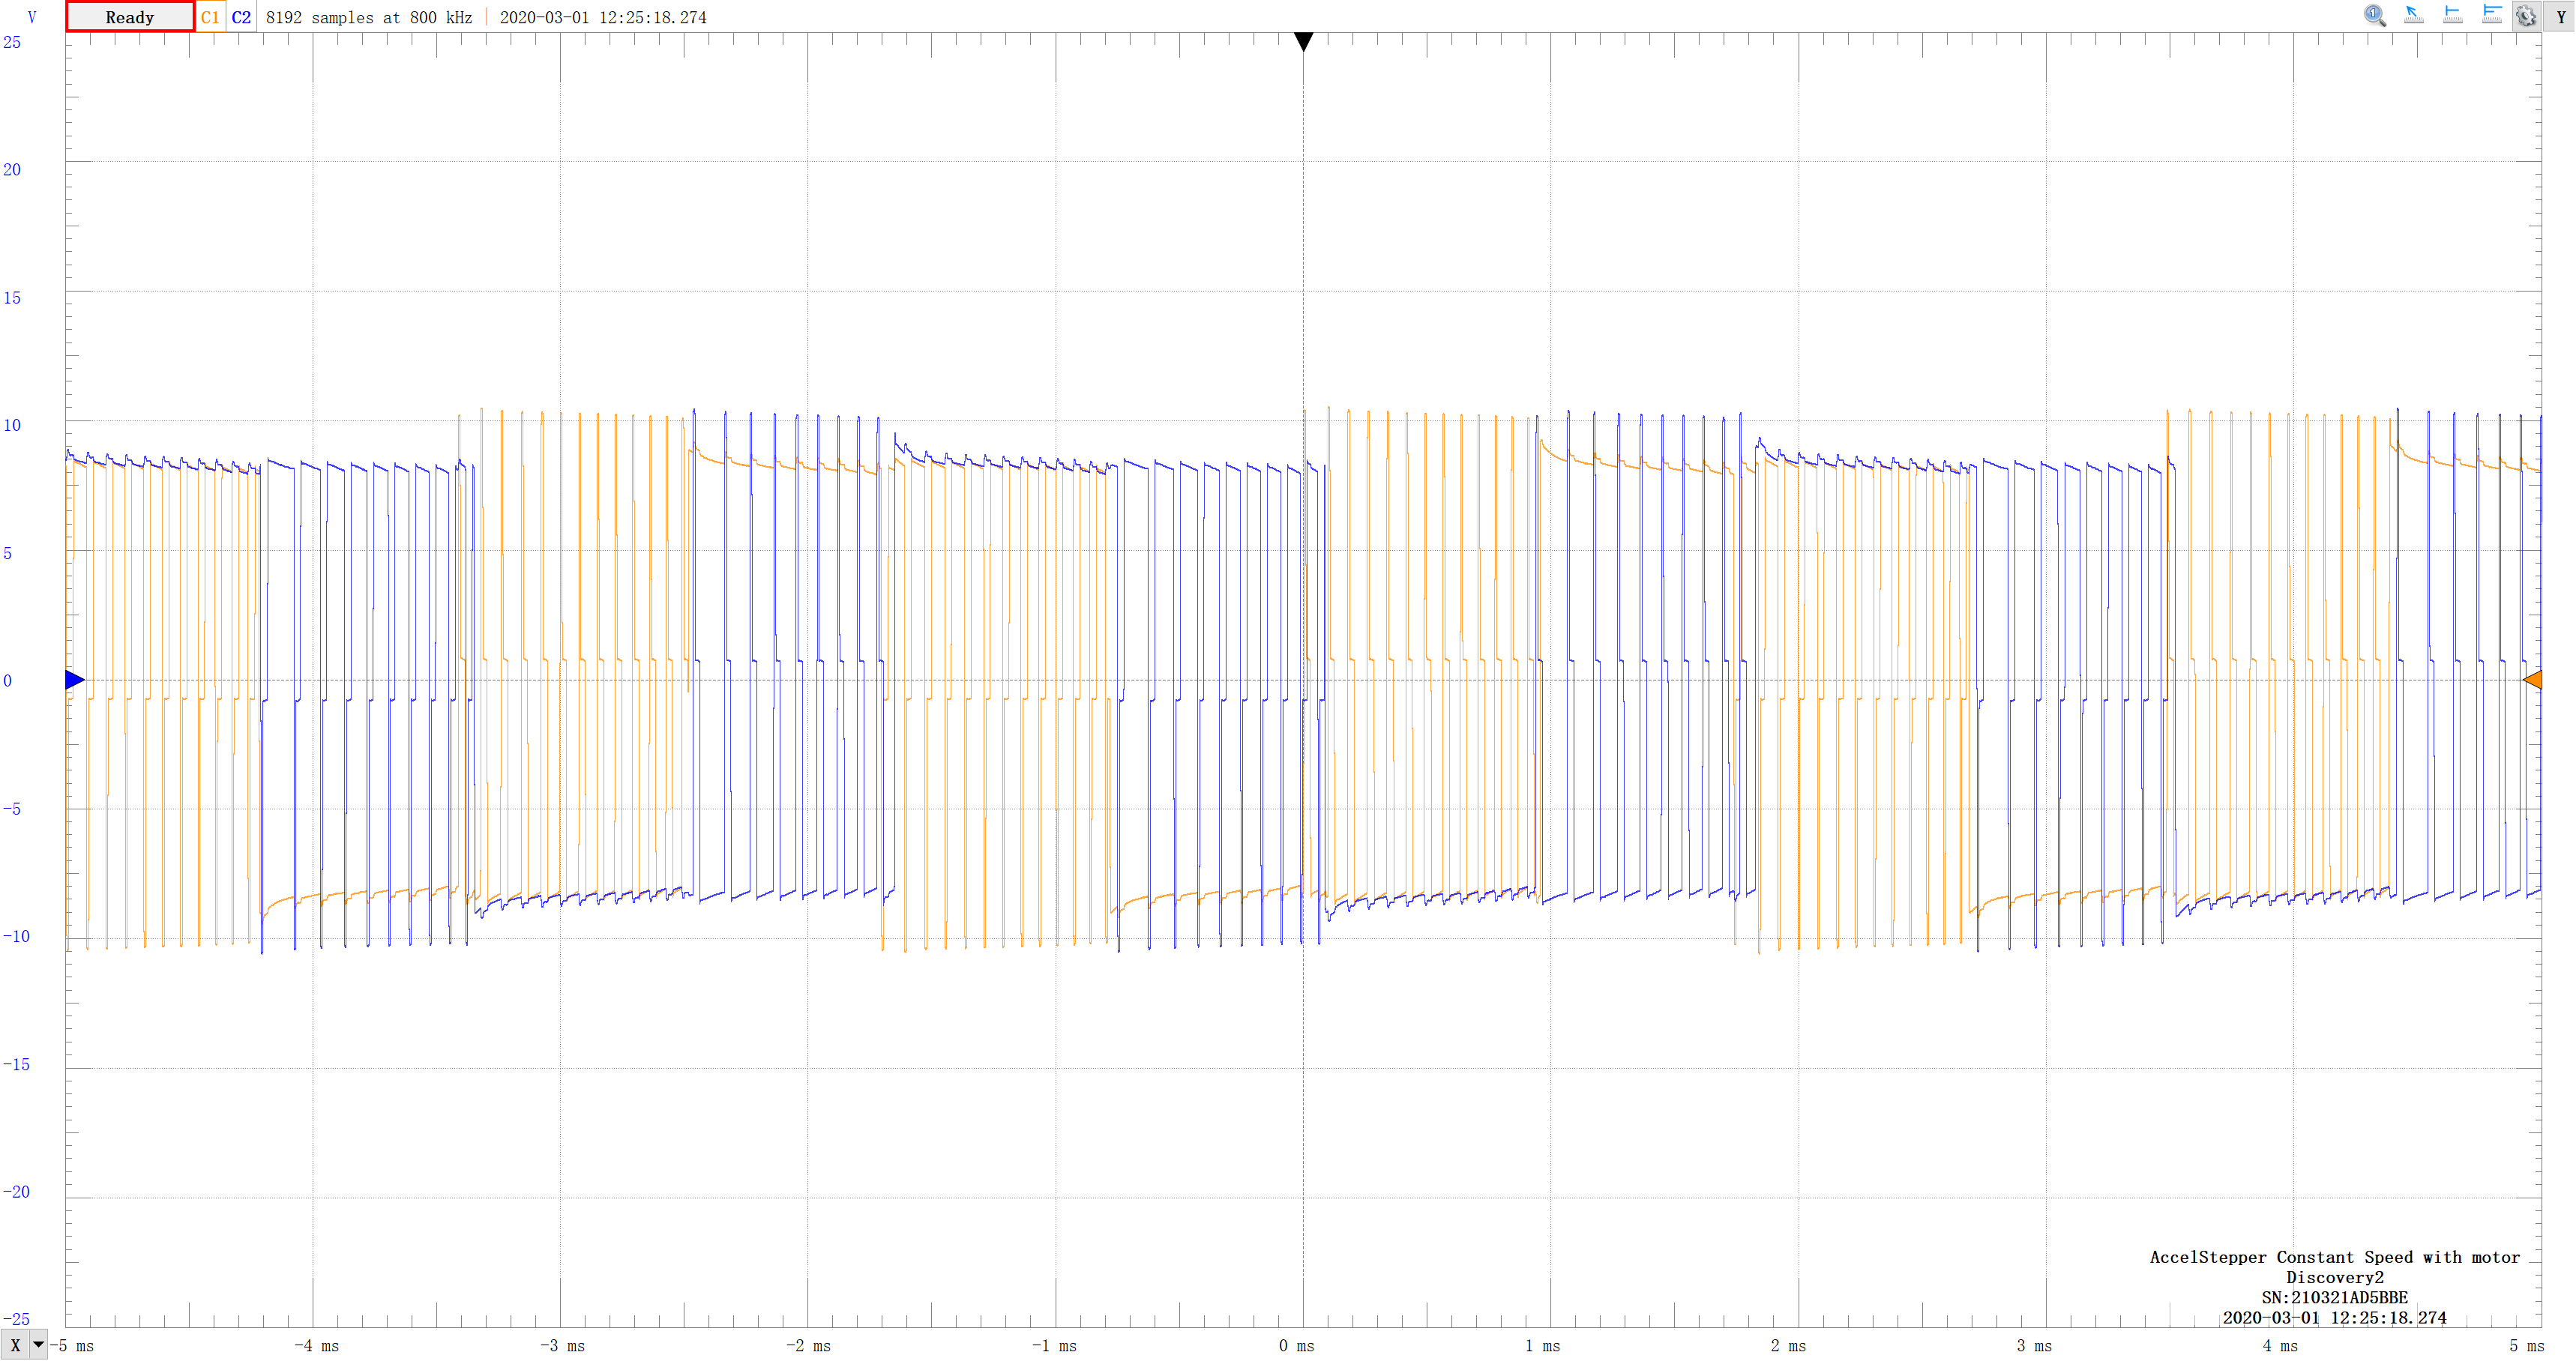
\includegraphics[width=\columnwidth]{AccelStepper-Constant-Speed-Waveform-with-motor.png}
    \caption{AccelStepper库恒速转动DRV8825接电机输出驱动波形}
    \label{fig:AccelStepper-Constant-Speed-Waveform-with-motor}
\end{figure}

\begin{figure}[htbp]
    \centering
    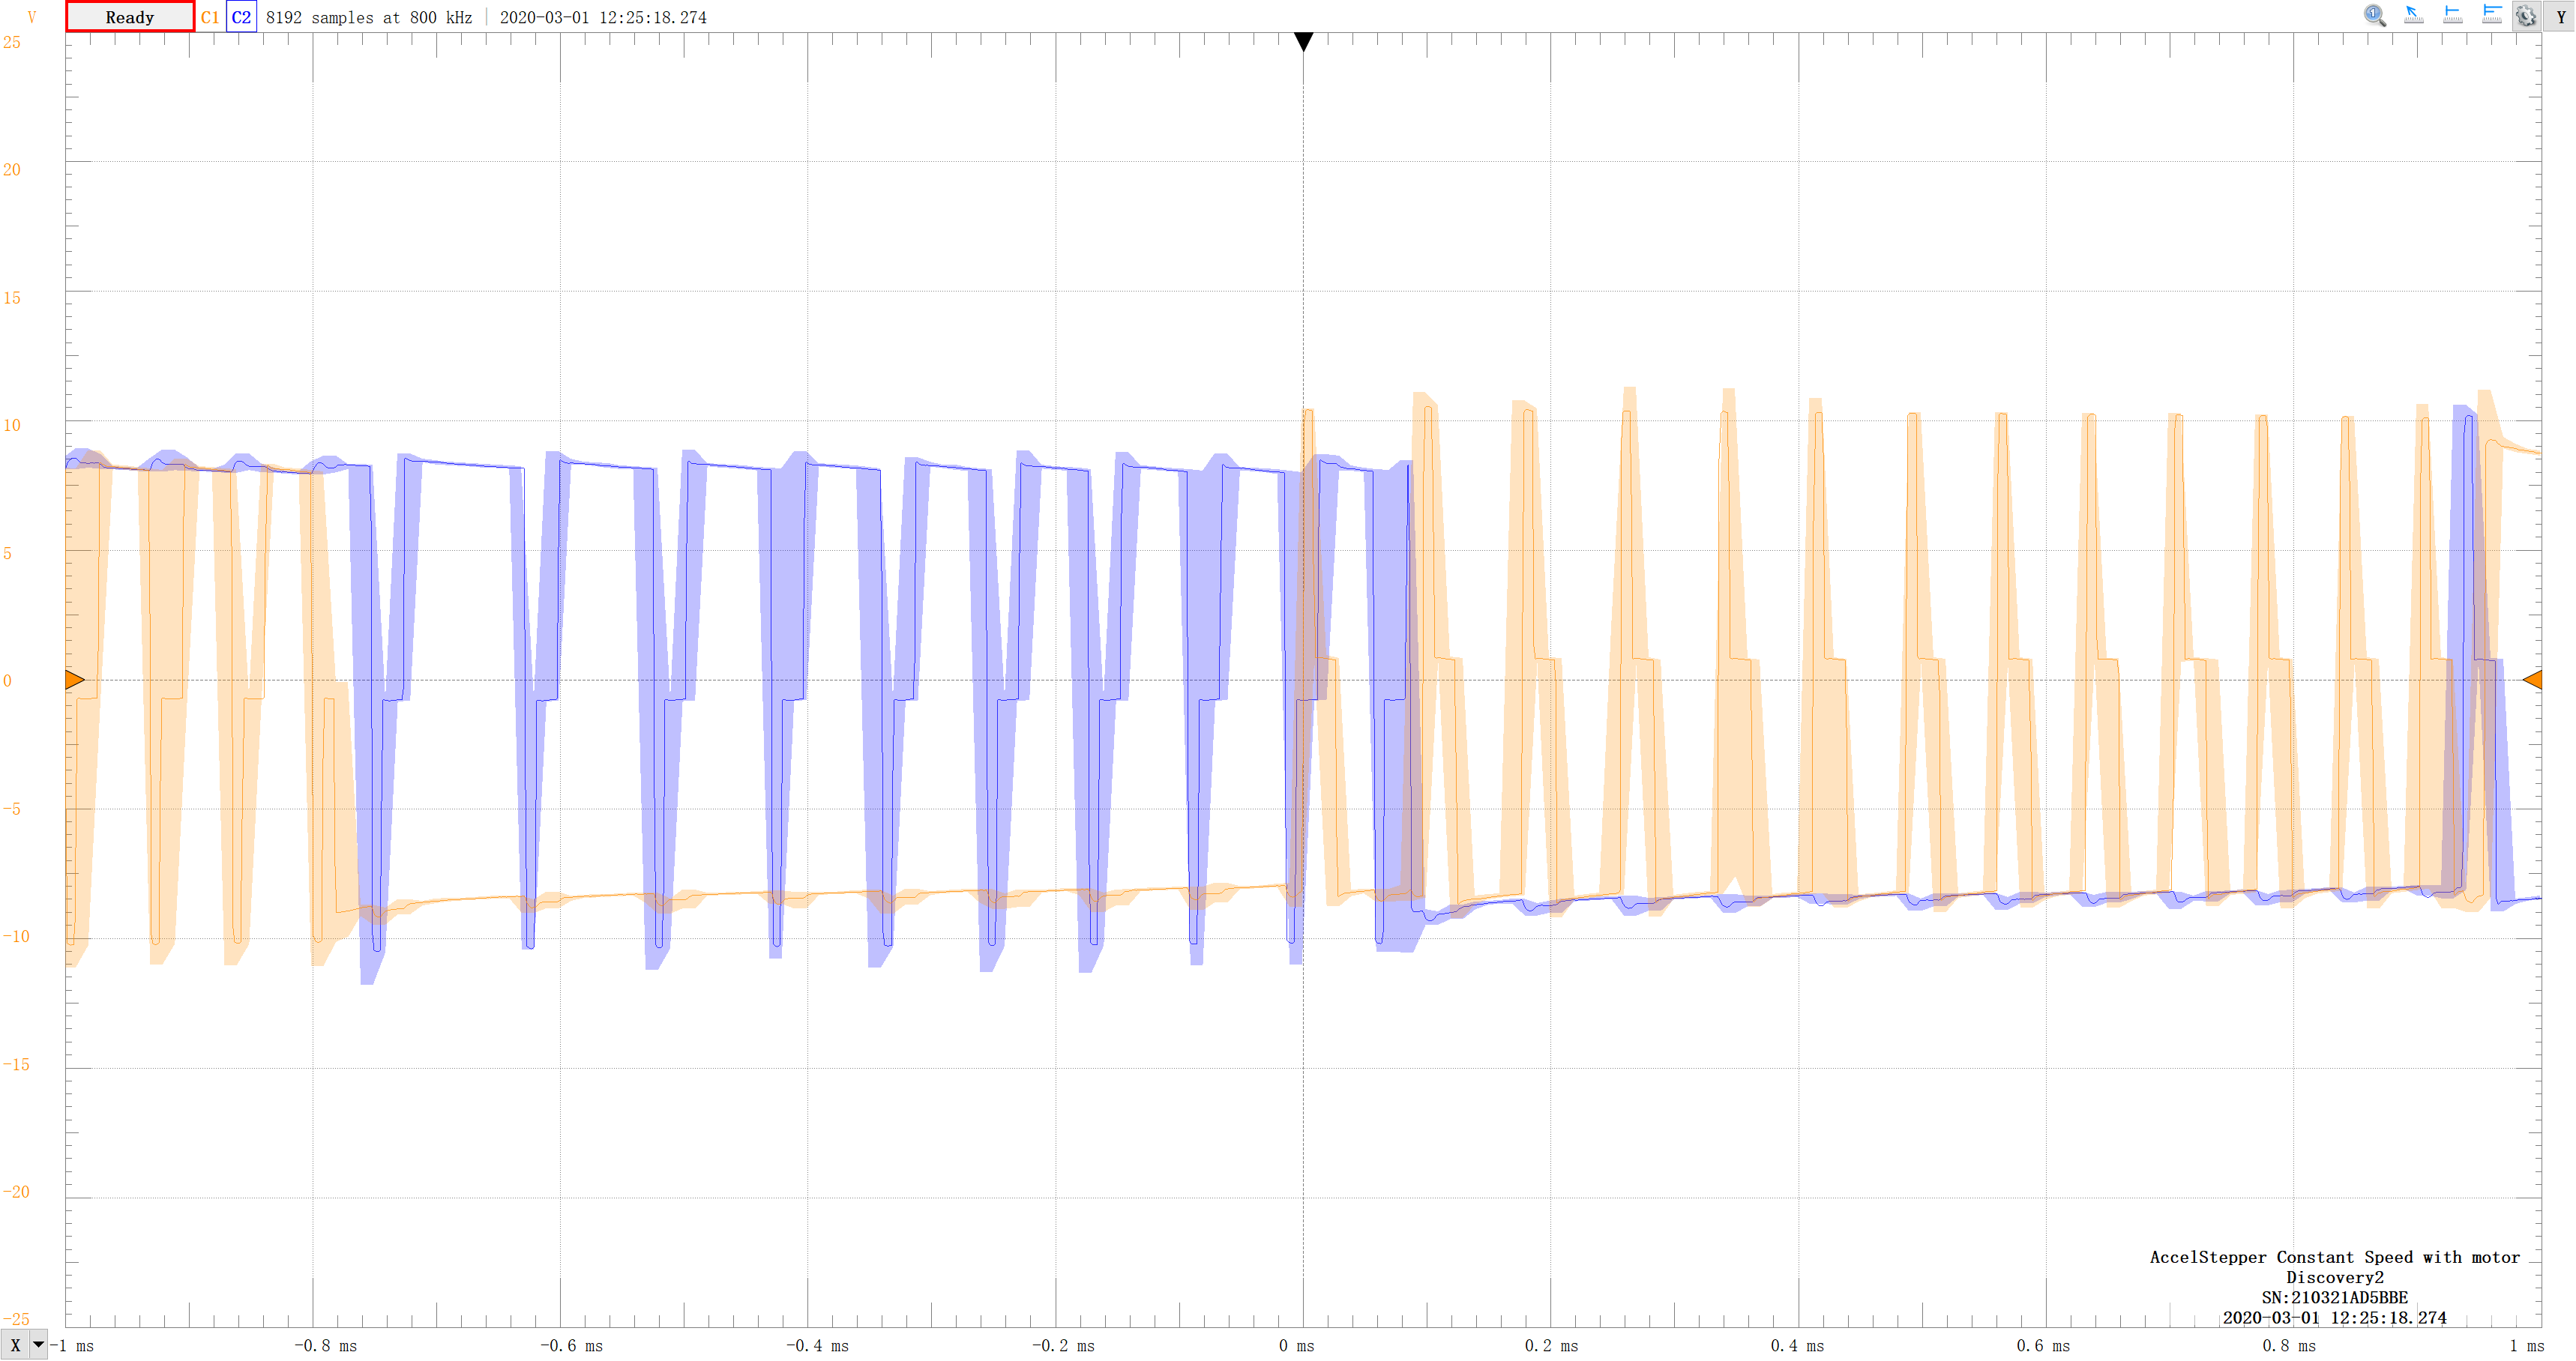
\includegraphics[width=\columnwidth]{AccelStepper-Constant-Speed-Waveform-with-motor-Scaled.png}
    \caption{AccelStepper库恒速转动DRV8825接电机输出驱动波形(放大)}
    \label{fig:AccelStepper-Constant-Speed-Waveform-with-motor-Scaled}
\end{figure}

\section{动力系统测试}

三电机在3D打印出的测试用底盘测试,以确定扭矩是否足够带动平台。